%***************************************************************************%
%                                  PREFACE                                  %
%***************************************************************************%
\documentclass[../main/main]{subfiles}
\begin{document}

% change prefix figure numbering/lettering
\renewcommand{\thefigure}{\Roman{chapter}.\Roman{figure}}
\renewcommand{\thetable}{\Roman{chapter}.\Roman{table}}

% prefix section heading
\renewcommand{\thechapter}{\Roman{chapter}}
\renewcommand{\thesection}{\Roman{chapter}.\Roman{section}}
\renewcommand{\thesubsection}{\Roman{chapter}.\Roman{section}.\Roman{subsection}}

\chapter{Preface}
%===========================================================================%
% SECTION
%===========================================================================%
\section{Talking about waste}
Waste has inherently been a poor subject for discussion, the term naturally cannotes disease, vileness, and ultimately death. Unfortunately these cannotations are true, improper handling and negligence of waste do lead to disease and death. As the World Health Organization has estimated in 2016, nearly 12.6 million deaths are associted with unhealthy environmnents and living conditions. In other words, 1 in 4 of total global deaths are caused by unhealthy living conditions primarily contributed to wasteful and negligent environmental practices~\cite{who2016}.

Ironically, the public perception of waste manifested from centuries of unhealthy and unsustainable waste management practices which gave rise to the associated maladies we describe waste today. Waste on its own is defined as materials eliminated or discarded from a used good or process. Be it excess materials, unwanted by-products, or goods that are consumed and transformed into an unwanted form. The subsequent dangers of waste: effluent, run-off, contamination, etc. are caused by a lack of sufficient handling and containment practices, and in extreme cases, active disregard for safe waste disposal. This meant discarding waste in dumps, landfills, and environmentally vulnerable locations. Until the 1920s, this laissez-faire approach for handling waste manifested into a global spread of contaminated areas. What we see today, waste as an abhorrent and dangerous entity, is the product of centuries of inaction leading to the ill-definition we describe it today.

The discussion of waste is also actively suppressed, as more salient news eclipse its much needed discussion. Instead, society has been more moved by discussions of emerging technologies, new feats in engineering, and cures for diseases. These topics do deserve their headlines, but underneath every achievement is the hidden mark of waste. For example, putting a cell-phone in every hand has given rise to a new form of waste, electronic waste (e-waste). E-waste is now one of the fastest growing waste streams with a global production of 45 million metric tons equating to 6 kg (13.2 lbs) of discaraded e-waste per person per year~\cite{balde2017}.

The environmental and health dangers of mining for raw materials, expanding manufacturing processes, and the short life-cycles of electronic goods~\cite{hong2015} is often not seen by the consumer and subsequently not a concern for industry. Also, establishing proper waste treatment practices can be harmful to a company's immediate revenue performance, and even with potential long-term gains in building environmentally friendly practices investment in cleaner technologies may not outweigh immediate performance metrics~\cite{king2001}. Likewise, industries are often defensive, sometimes employing political or marketing tactics to circumvent new environmental policies. In some cases, policies are ignored completely~\cite{nemerow1998,markowitz2013}. For example, in 2013 Wal-Mart was accused and pleaded guilty of illegally dumping hazardous waste, almost 2 million pounds of pesticides in protected areas from 2006-2008~\cite{usatoday2013}, despite laws inacted to prevent this. There are many more examples of companies that have attempted to circumvent waste management laws, when in 2009 the New York Times cited that within their 5 year investigation almost 500,000 cases of illegal industrial waste practices were performed~\cite{duhigg2009}.
Even on a city-wide scale, events such as the Flint water crisis and West Virgina chemical leak, both occured in 2014, are still struggling to remediate their contaminated drinking waters because of slow moving politics and inadequate waste management infrastructure~\cite{haimerl2017,kristabryson2016}.

This work is intended to not only show new waste management technologies, but to also encourage the conversation about our current state of waste. The goal is to overcome the first barrier preventing productive waste management initiatives, and that is to acknowledge it as a problem.

%-----------------------------------------------------------------%
% SUBSECTION
%-----------------------------------------------------------------%
\subsection{Waste -- a historical context}
Government waste management practices in the United States did not exist until the early 1800s~\cite{elliott2013}. Since then, the main waste management practice tacitly followed two principles. The first was to remove waste out of public sight, and the second was a belief that nature or some other entity would eventually deal with it~\cite{elliott2013}. These two mentalities were the hallmark of the Industrial Revolution (circa 1760-1840), in which waste was seen as an annoyance that interferred with productivity~\cite{williammcdonough1998}. However, as manufacturing and production grew, so did waste. The quantity of waste, whether it was manufactured by-products, excess chemicals, biological waste etc. were routeinly discarded hapharzardly on the streets, buried, or dumped into nearby streams. It was not until the 1880s that waste became visibly obvious. Streets were dirty, waters were soured, and the connection between illnesses and waste became synced in the public's mind~\cite{louis2004}.

Unfortunately, because municipal waste was disregarded for almost a century, there existed no waste management infrastructure and almost no government investment to build one~\cite{elliott2013}. In a reluctant series of finger pointing, the eventual clean up responsibility fell on to the city---but only loosely. Transitioning into the 1900s the municipal government assumed primary responsibility for solid waste streams produced at the local level and established related services such as collection and disposal. Industries on the other hand were held self-accountable of their hazardous waste~\cite{elliott2013}.
Despite the switch to actively manage waste, there was no capital to build new waste management infrastructure, and sometimes building such infrastructure was insurmountable given city constraints. So solid waste management primarily relied on establishing municipal dumps where waste was collected and stored, with the hope that future technologies would eventually process it~\cite{louis2004,elliott2013}.

Local municipals took the burden of finding and establishing new dumping grounds, and industries continued their laissez-faire approach when managing their own. Given the separation of responsibilities there were often clashes when state or federal legislations implemented new waste management regulations. % forced break

%======================%
% waste accumulation
%======================%
\begin{figure}[H]
	\centering
	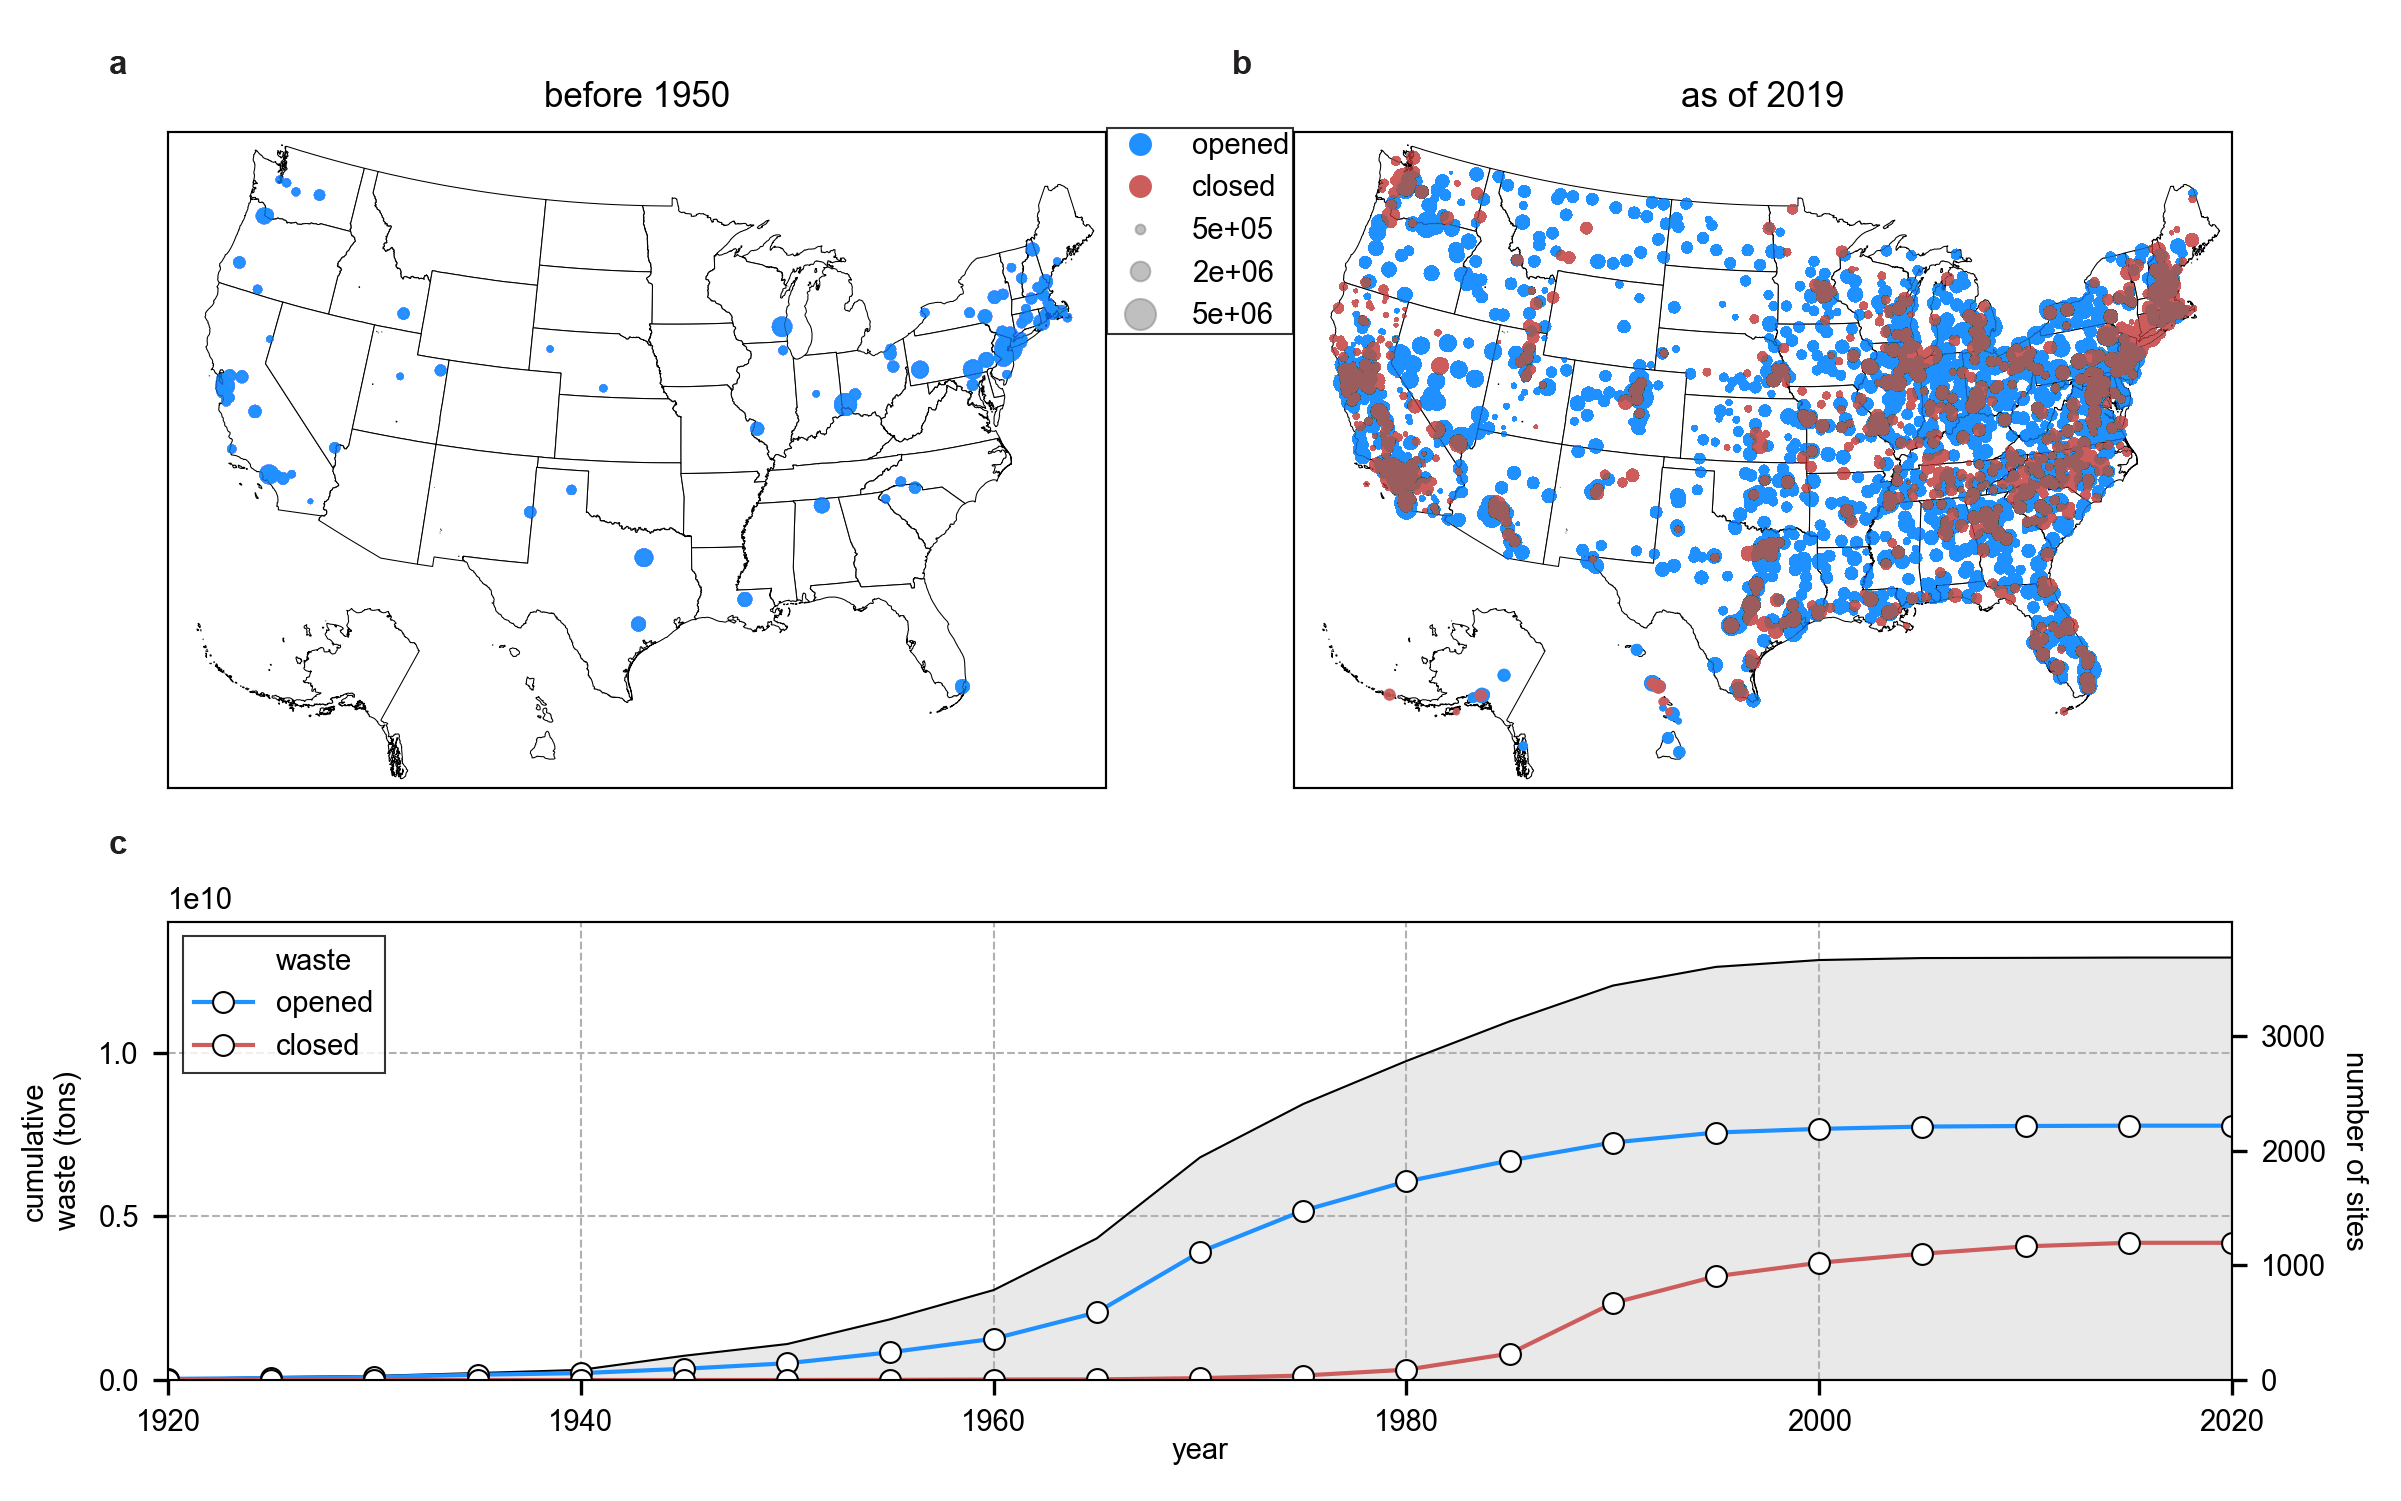
\includegraphics[width=\linewidth]{lmop-usa-map.png}
	\caption[Mapping and number of landfills in the United States from 1950 to 2019]
	{
		\textbf{Mapping and number of landfills in the United States from 1950 to 2019}\protect\footnotemark.
		(\textbf{a}) A map of the United States indicating locations of landfills during the first recorded year in 1950. Blue sites indicate opened (during that time), and radius of site corresponds to the amount of waste produced.
		(\textbf{b}) The same mapping in 2019. Blue indicates opened sites, and red indicates closed sites.
		(\textbf{c}) More than 10 billion tons of accumulated landfill waste had been discarded on United States' soil since reporting began in 1920. The rate of waste production accelerated between the 1960--80s; however, the production has slowly plateaued to a rate of >250 million tons per year~\cite{usepa2017b}.
  }
  \label{figure:preface:lmop-usa-map}
\end{figure}
\footnotetext{
  USA landfill and geolocation data available at: \url{https://catalog.data.gov/dataset?metadata_type=geospatial&_metadata_type_limit=0&q=Landfill}
  \linebreak
  USA landfill sites by the year available at: \url{https://www.epa.gov/lmop/landfill-technical-data}
}

\noindent Industries would lobby for looser control and less oversight, hoping to keep their manufacturing practices unperturbed. The outcome was ineffective regulations that focused on specific waste streams rather than broadly tackling the overall inefficient waste process~\cite{markowitz2013}. Many loopholes existed allowing many industries to continue their unregulated dumping. Rather than placing new guards around unsustainable waste practices, new legislation instead provoked the rise in organized resistance and industrial lobbying~\cite{elliott2013,markowitz2013}.

Consequently, regulation of waste disposal did not consistently occur at the municipal, state, or federal level until the 1960s. At that time the quantity of waste became physically impossible to avoid, and the public soon became aware of its daunting health and environmental consequences. In the 1950s, there were 74 municipal landfills across the United States, each on average containing more than 1.2 million tons of waste~(\FIGURE~\ref{figure:preface:us-timeline}). Within 10 years, the number of landfills more than doubled to 192 sites.

Public awareness and activism was also spurred by the ongoing social and civil rights movements. The momentum for transforming public opinion into political initiatives also pushed environmental protection and sustainability legislation into the government agenda~\cite{cutter1995}. Especially, the book Silent Spring by Rachel Carson (1962) also contributed to a social movement for environmental protection and subsequently helped enact actionable policies, namely the Clean Air Act in 1963 and the eventual formation of the National Environmental Policy Act in 1969. Municipal waste management (MSWM) activities finally received defining legislation in 1976 through the Resource Conservation and Recovery Act (RCRA) which forced closure of open dumps and required regional planning of municipal waste~\cite{louis2004}.

However, these policies had their loopholes and negative repercussions. With the closing of municipal dumps, waste had to be transported elsewhere such as dedicated processing plants. Unfortunately, handling transportation of waste, the involved labor cost, and the potential tax implications of moving waste between state lines\footnote{
	waste was now defined as a good of commerce by the United States' Supreme Court under the Commerce Clause of the Constitution~\cite{louis2004}
}, made waste processing much more logistically challenging. Therefore, waste was still largely handled by municipalities, and often municipals would contract private companies to move waste between facilities or statelines much like exporting or importing a good.

The net result was exactly the same as before but on the national level, the movement of waste between state lines to government owned landfills~\cite{elliott2013}. Unfortunately, the growth in waste regulation from 1960-1990 did not correlate to a reduction in waste or improved waste management~\cite{andrews2018}.

%======================%
% waste timeline in US
%======================%
\begin{figure}[H]
	\centering
	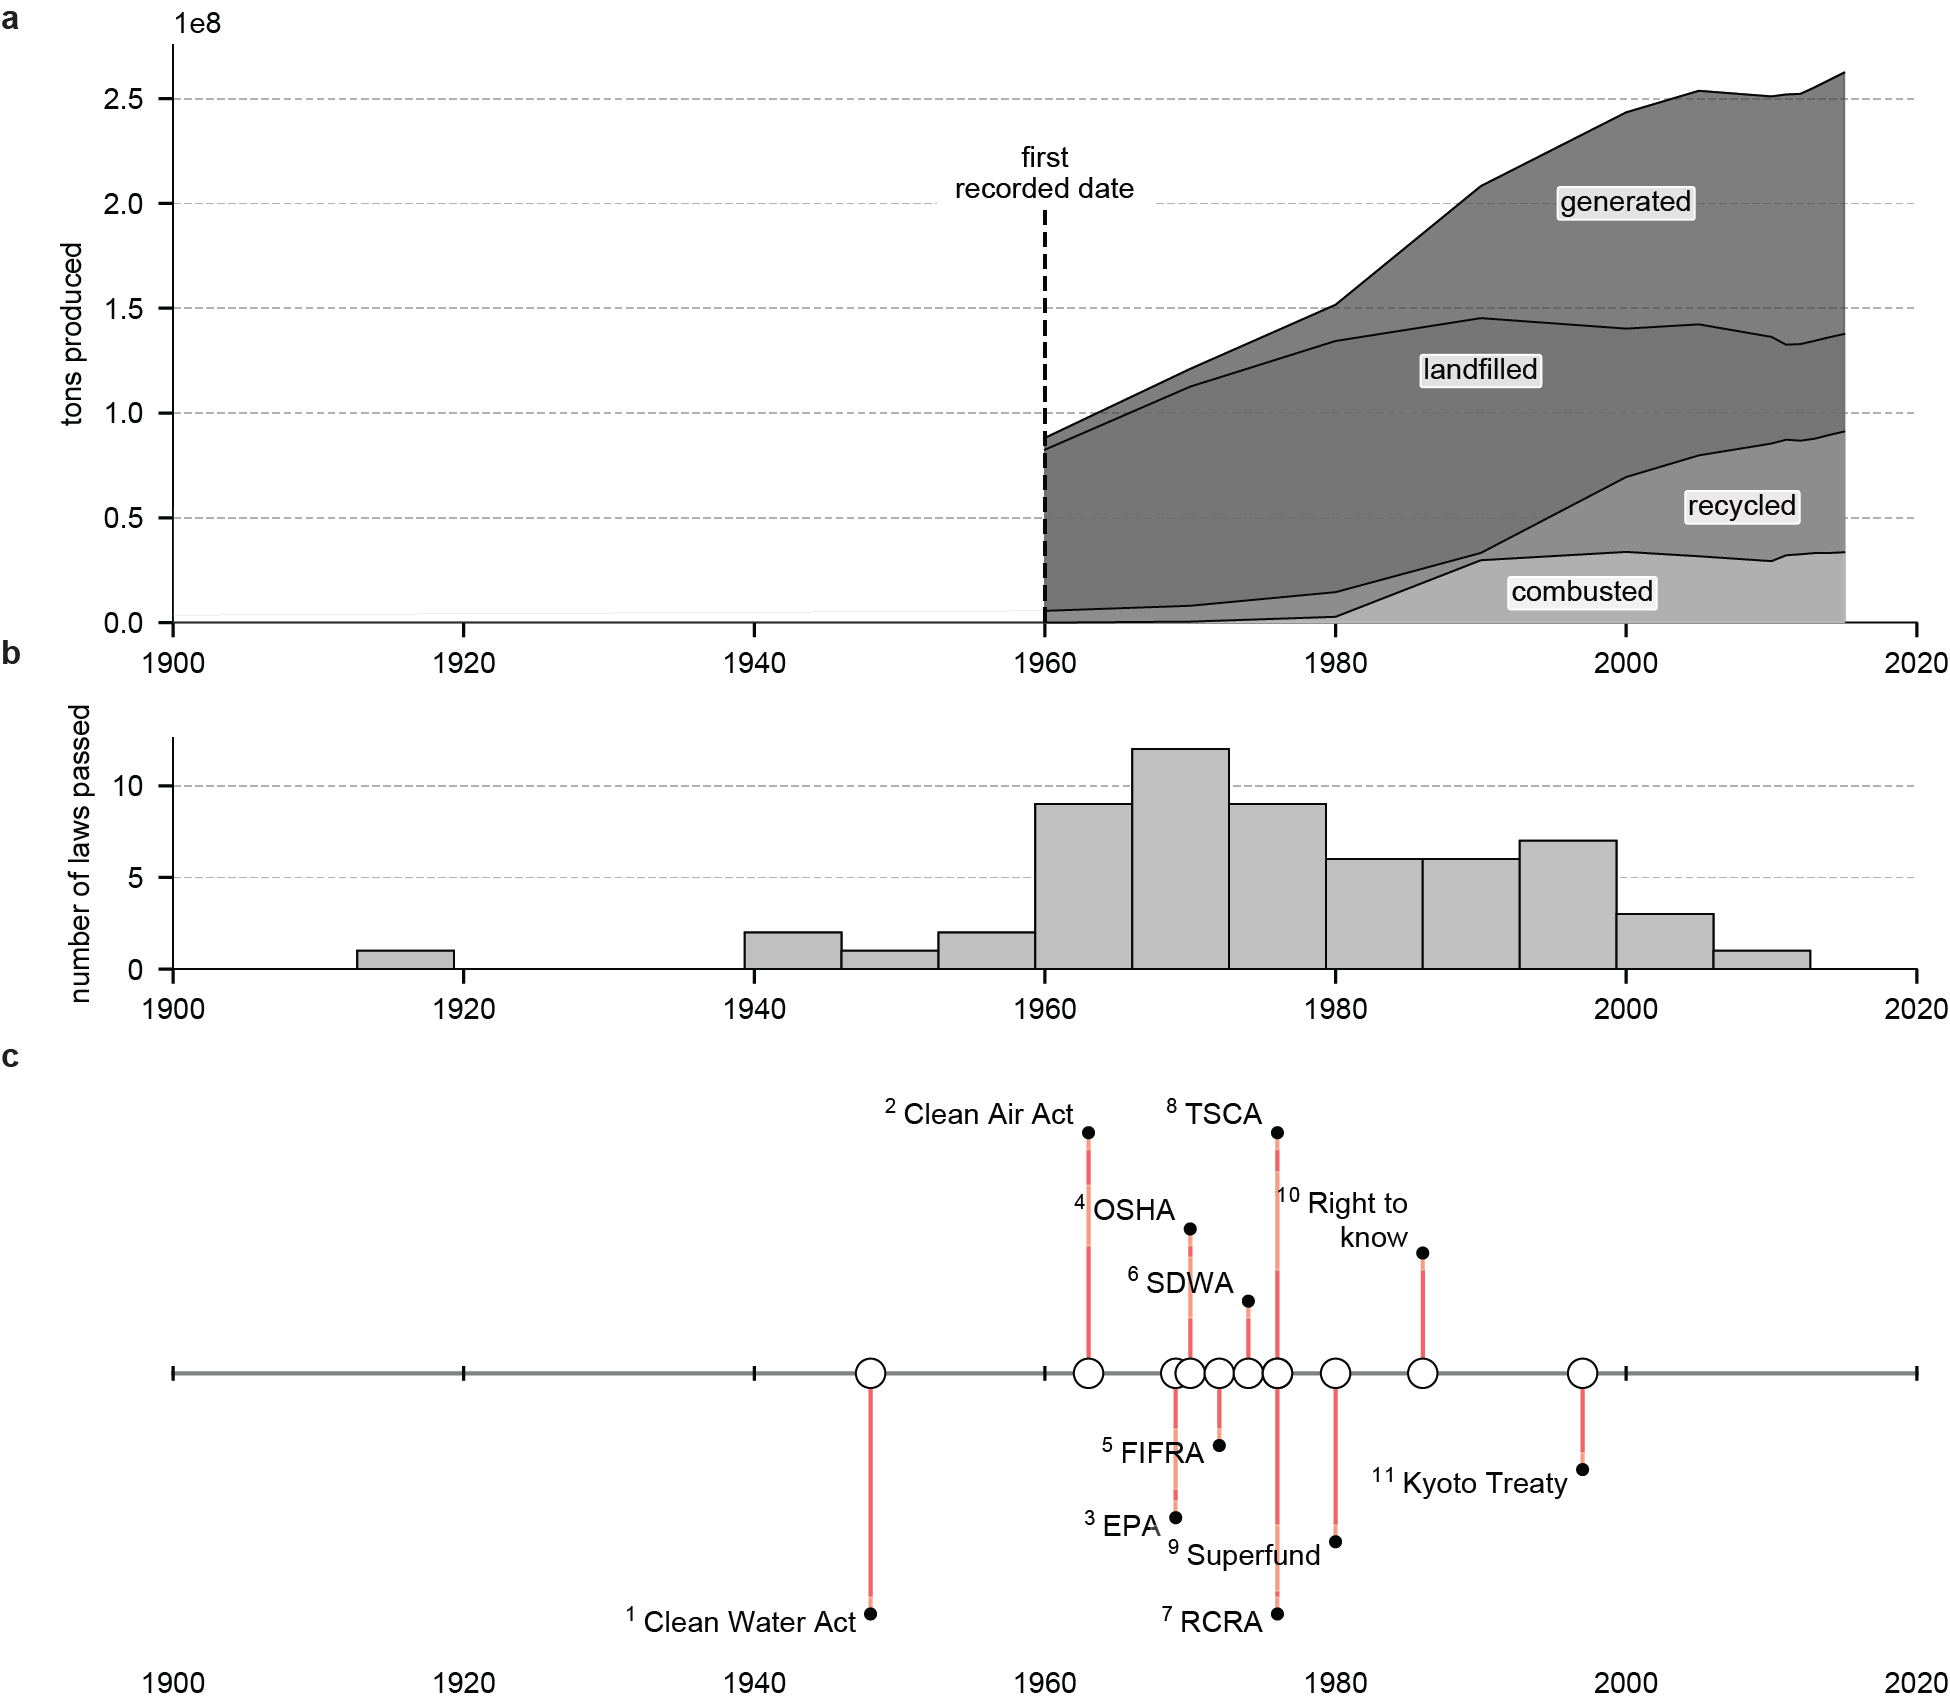
\includegraphics[width=\linewidth]{MSW-timeline.png}
	\caption[The rise in waste and government policies]
	{
		\textbf{The rise in waste and government policies}\protect\footnotemark.
		(\textbf{a}) The growth of recorded municipal waste since 1960 until 2016. The shaded regions breakdown the total generated waste into landfilled, recycled, or combusted (burned).
		(\textbf{b}) A histogram indicating the breakdown of waste related legislation in the United States starting as early as 1910 to 2019. There were more than 57 major legislative actions concerning waste starting in 1916, with a spike in 1960 during the passing of the Clean Air Act and the EPA. The number of legislation has reduced since the 90s, as legislation at the state and federal level have more relied on global NGO initiatives (e.g. WHO, UNEP, etc.) which has now become the governing body for waste management policies.
		(\textbf{c}) Highlighted environmental policies enacted that laid the groundwork for waste management in the United States.
  }
  \label{figure:preface:us-timeline}
\end{figure}
\footnotetext{
  USA wastestream type and quantities: \url{https://catalog.data.gov/dataset/sustainable-materials-management-smm-materials-and-waste-management-in-the-united-states-key-f}
  \linebreak
  list of EPA policies: \url{https://en.wikipedia.org/wiki/Environmental_policy_of_the_United_States}
}

% break
\noindent  In the 1990s, disposal of hazardous waste increased by 25\% \cite{usepa2015,usepa2017b,andrews2018}.
Loopholes and exemptions encouraged waste generators to dilute their waste with nonhazardous waste streams and incentivized cheating or mis-reporting numbers. Overall, the rise in environmental laws did not curb the amount of waste or disincentivize illegal practices (\FIGURE~\ref{figure:preface:lmop-usa-map})~\cite{elliott2013,colten2010}. To this day, the result is more than 2000 active and 1000 closed or abandoned landfill sites. Many of the abandoned sites still contain waste and have yet to be properly remediated. Currenlty, the United States produces more than 250 million tons of waste per year~\cite{usepa2017b}, which is equivalent to approximately 4.5 pounds per person per day~(\FIGURE~\ref{figure:preface:lmop-usa-map}).

The villainization of waste was not because waste was inherently thought of as an evil entity, as for almost two centuries waste was mostly viewed as an inconvenience. Instead, the villainization of waste grew through the insufficiency of cities and indifference of industries that allowed waste to grow to an unmanageable quantity we see today. Today's anxiety about waste production and waste management is warranted, but only because waste has now accumulated to a point that is impossible to ignore.

%-----------------------------------------------------------------%
% SUBSECTION
%-----------------------------------------------------------------%
\subsection{Waste -- current perspectives}
To understand the current and future implications of waste and its growing new forms, a societal picture should be examined to explain how changing moods and public opinion could have a profound impact on waste management decisions. A growing number of literature concerned about a new age of modernity was written as a reaction to the techno-social revolution from the 90s onwards. This techno-social revolution was seen as an increased interconnectivity between countries, industries, and people~\cite{ekberg2007}. This body of literature suggested that society had entered a new modernity, where nations were no longer bound by geographical lines and risks were inherently made in everyday geopolitical decisions. A framework to view this shift in societal behavior was pioneered by Anthony Giddens, Scott Lash, and Ulrich Beck's theory of the ``risk society''~\cite{elliott2013,giddens1991,beck1992}. In their definition, a risk society is mainly concerned about future goals, whether policies, technologies, or shifts in public opinion. Society is reactionary rather than preemptive or anticipatory to the risk involved, be it changes in government, the scientific community, or environmental health.

For example, the rise in gene editing technologies have faced morale and ethical questions~\cite{wang2019}, yet the scientific advancement of the technology will continue forward until more tangible consequences emerge. Unfortunately, these ``tangible consequences'' are ill-defined and are often manufactured in an attempt to provide substance to a future unknown. Contrary to the era of the industrial revolution, risks/concerns were mainly revolved around tangible and quantifiable items, such as products and distribution of goods. In a risk society, risks are conceptual and ultimately manufactured given expectations and opinions. These are called ``manufactured risks''. To continue the example, a manufactured risk for gene editing technologies would be the possibility of abusing genetic modifications to unfairly enhance success (beauty, intelligence, immunity, etc.). Other day-to-day manufactured risks may be whether companies will remain solvent, rise and trade of investments and stocks, and the hope of emerging technologies such as new therapeutics or quantum computing to alleviate current stresses (e.g. diseases and aging technologies)~\cite{beck1994,beck2006}.
This concept goes beyond technology to ecological disaster, diseases and epidemics, population growth, food and water limitations, and territorial conflicts~\cite{beck1994,elliott2013}. Many of these manufactured risks have no historical reference to provide estimation, so they are largely unpredictable.

In Gidden, Lash, and Beck's discussion, societies reflexive response to risk shapes the new modernity, in other words, ``reflexive modernization''~\cite{beck1992,beck1994}. Reflexive modernization is a main characteristic of risk societies, that is concerns (i.e. risk) are focused on large-scale techno-scientiic processes pursued by industralists, engineers, and policymakers while equally downplaying the negative repurcussions of such actions in order to emphasize economic growth and convey a sense of progress. Given these concepts of reflexive modernity, the rise in risk societies, and the creation of manufacturered risk, there are three main conclusions that can explain today's loose and reluctant behavior in addressing the current waste crisis. The first is that globalization has made risk societies extend beyond geographical borders. Risks are now shared between countries, and risks such as waste is increasingly burdened onto transnational forces such as corporations and NGOs like the United Nations and World Health Organization rather than the nations themselves. The second is the re-definition of waste as a manufactured risk. When speaking about waste, it is no longer an object or a thing, but a concept. Rather than handling the current physical mass of waste, policies are aimed at reducing the notion of waste as a harm to society. Statements such as ``zero-discharge'' and ``zero-emission'' are intended to convey a proactive stance on waste management, even though producing zero waste is nearly impossible for any process~\cite{wang2004}. Lastly is the question of who is responsible. As waste is now interpreted as a manufactured risk, it is easily passed through multiple hands with varying degrees of interest. Ironically, it is the same political, business, and scientific expertise which are called upon to answer the problems of earlier wasteful trends generated from previous political, business, and scientific actions~\cite{beck1992}. Examples would be the concern over nuclear waste and plastic waste, which prior to their now known environmental hazard, were used freely without much regard about their disposal. As these same politicians, businessmen, and scientist are more concerned about progress, the nature of this risk is slowly dissipated through cursory arguments leaving the public more entertained by other concerns such as the internet, new technologies, and the economy~\cite{andrews2018}.

%-----------------------------------------------------------------%
% SUBSECTION
%-----------------------------------------------------------------%
\subsection{Waste -- current and future trends}
\label{section:preface:current-and-future-trends}
Past actions (or inactions) towards waste and the transition into the reflexive modernity suggest that society as a whole reacts to waste rather than actively managing or preemptively preparing for it. Align with the concept of the risk society, many nations are more concerned with growth, namely the developing world such as China, India, South American, and African countries~\cite{cohen2006urbanization}. Trends in a country's population and gross domestic product (GDP), preliminary metrics to estimate a country's growth, can be correlated with waste production to help elucidate the relationship between a country's development and waste output. Data from 2017 on population, GDP, and waste production of 217 countries, broken down to high and low economic groups, were fitted with a linear model. An increase in population and GDP, irregardless of economic status, correlates strongly with an increase in waste production~(\FIGURE~\ref{figure:preface:global-waste-trend}). Particularly, high income countries (HIC) have a higher ratio of waste production per capita, on average generating 69 tons of waste per thousand citizens.
Whereas for low income countries (LIC), as well as upper and lower-middle income countries (HMC and LMC, respectively) waste production is almost 5 times less per capita~(\TABLE~\ref{table:preface:trend-pop-gdp}a).

%==========================%
% Scatter plot waste gloabl
%==========================%
\begin{figure}[H]
	\centering
	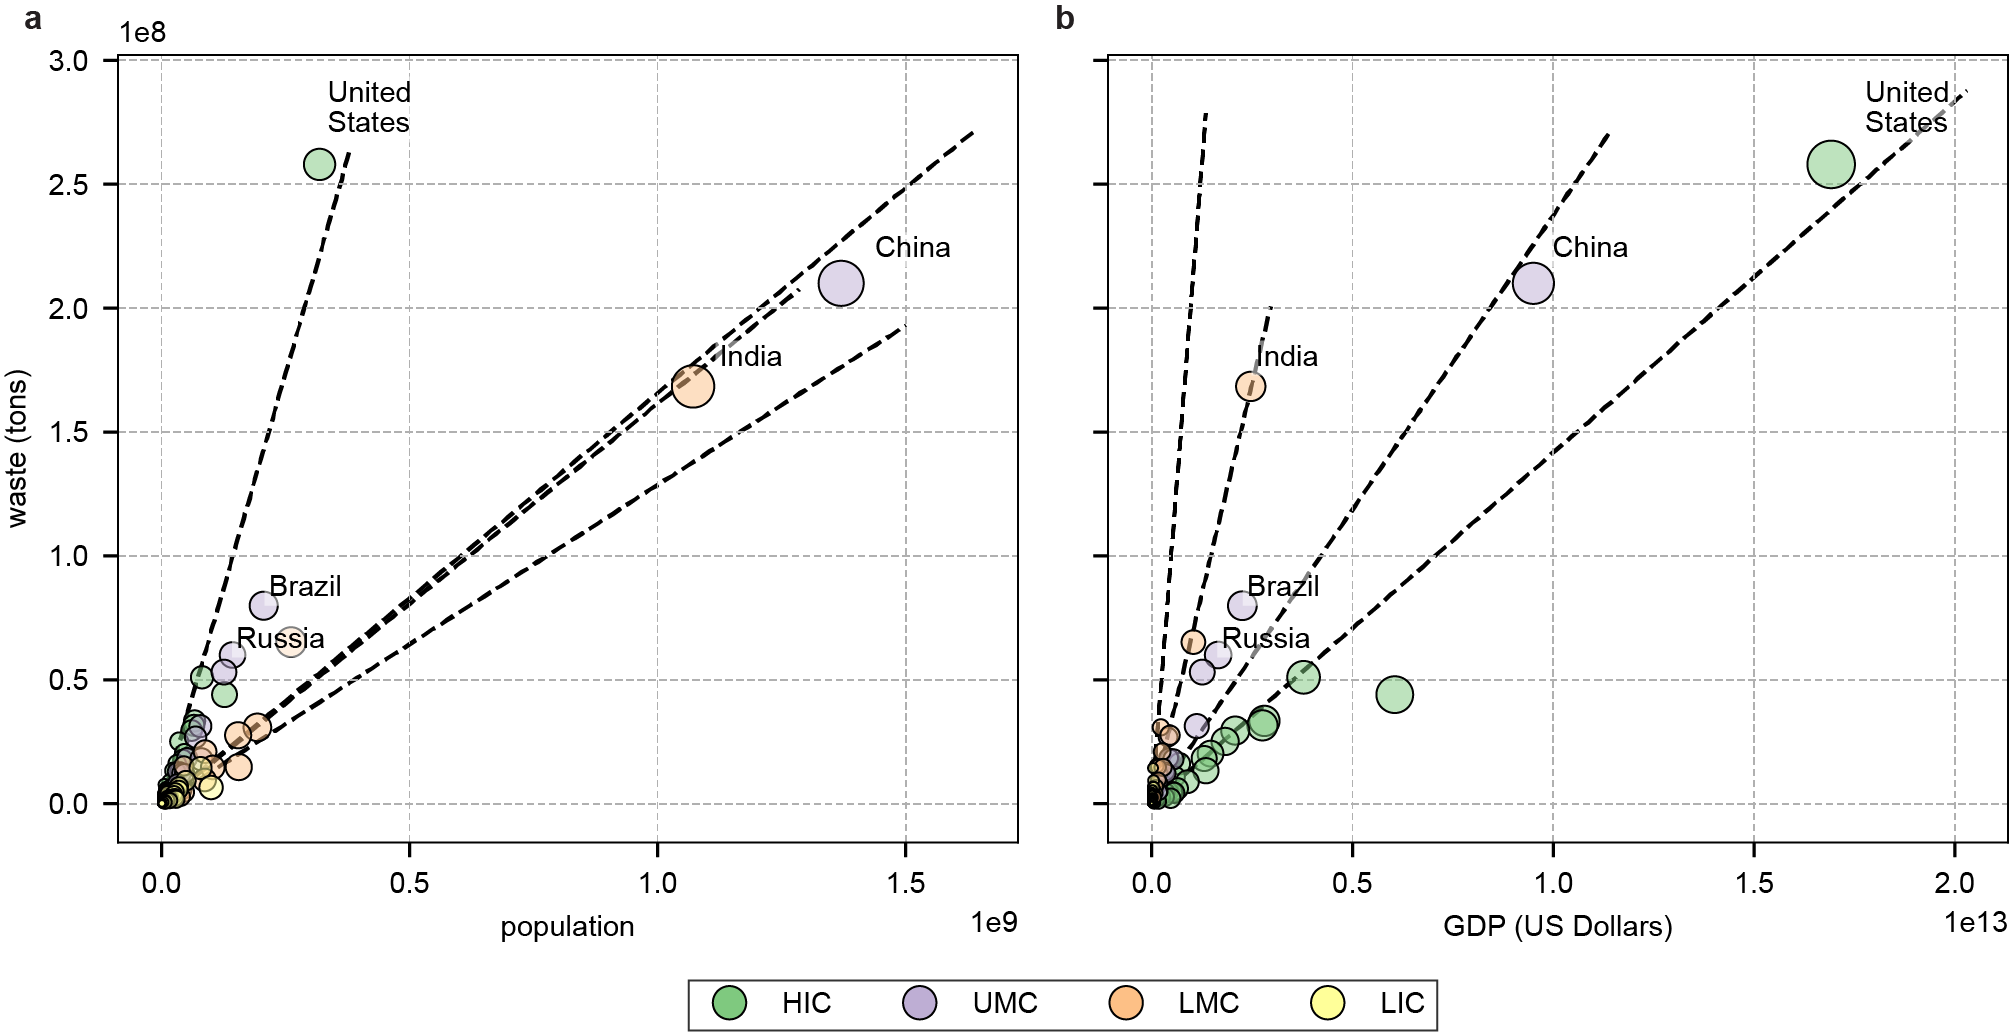
\includegraphics[width=\linewidth]{global-waste-trend.png}
	\caption[Correlation between waste production and population \& GDP for 217 countries, broken down by economic status]
	{
		\textbf{Correlation between waste production and population \& GDP for 217 countries, broken down by economic status}\protect\footnotemark.
		HIC = high-income country
		LIC = low-income country,
		LMC = low-middle income country,
		UMC = upper-middle income country.
		(\textbf{a}) Trendlines fitting waste production against country population levels as of 2017.
		(\textbf{b}) Trendlines fitting waste production against country GDP (normalized against the US dollar) as of 2017.
	}
	\label{figure:preface:global-waste-trend}
\end{figure}
\footnotetext{
  world population data available at: \url{https://data.worldbank.org/indicator/SP.POP.TOTL} \\
  world GDP data available at: \url{https://data.worldbank.org/indicator/NY.GDP.MKTP.CD?year_high_desc=false} \\
  global municipal waste data available at: \url{https://datacatalog.worldbank.org/dataset/what-waste-global-database} \\
	classification of countries based on economic status: \url{http://faculty.ucr.edu/~jorgea/econ181/wdr_2008.pdf}
}

Looking at the waste relationship with GDP, lower income countries such as India, Brazil, and China produce more waste per GDP than HICs such as the United States~(\TABLE~\ref{table:preface:trend-pop-gdp}b). This may suggest that countries with higher economic income can afford, or become more educated, on the impacts of waste and have the social and financial bandwidth to make the appropriate policy or technological changes.

%~~~~~~~~~~~~~~~~~~~~~~~%
% table on correlations
%~~~~~~~~~~~~~~~~~~~~~~~%
\begin{table}[H]
\small
\centering
	\begin{subtable}{.48\linewidth}
		\centering
		\caption{}
		\begin{tabular}{P{1cm} P{3.5cm} M{1.5cm}}
	\toprule
	    & tons per 1000 people
			& $R^2$    \\
  \midrule
		HIC & 69.4 & 0.94  \\
		UMC & 16.6 & 0.91  \\
		LMC & 16.1 & 0.97  \\
		LIC & 12.8 & 0.68  \\
	\bottomrule
\end{tabular}

	\end{subtable}
	% new line
	\begin{subtable}{.48\linewidth}
		\centering
		\caption{}
		\begin{tabular}{P{1cm} P{3.5cm} M{1.5cm}}
	\toprule
	    & tons per million \$
			& $R^2$    \\
	\midrule
		HIC & 14.2 & 0.96  \\
		UMC & 23.7 & 0.96  \\
		LMC & 67.8 & 0.99  \\
		LIC & 206  & 0.59	 \\
	\bottomrule
\end{tabular}

	\end{subtable}
	\caption[Regression model parameters on waste production as a function of population or GDP]
	{
		\textbf{Regression model parameters on waste production as a function of population or GDP}.
		(\textbf{a}) Fits between waste production and population level suggest that HIC countries produce more waste per capita. Units are in tons per thousand people.
		(\textbf{b}) Countries with higher GDPs, such as the United States, correlate to less waste production (HIC < UMC < LMC < LIC). Units are in tons per million US dollars.
	}
  \label{table:preface:trend-pop-gdp}
\end{table}

A similar trend discovery experiment can be performed for more country-specific metrics such as the level of urbanization, government budget (e.g. EPA), and the advancement of technology (e.g. Moore's law, pre-2010). A multi-variate time-dependent cross correlation on waste production versus these other metrics was performed for the United States. An analysis on the United States' waste trend could help foreshadow the trajectory of waste production for other countries such as China, India, and Brazil; countries that are currently encountering similar growth challenges the United States once did in the past decades.

Waste output for the United States has grown by 3.6 million tons per year, equivalent to 2 kilograms (4.5 pounds) of waste per person per day~\cite{usepa2017b}. This trend was cross-correlated with time-series for population growth, GDP, rise in technological power (indirectly through transister counts), and percent urbanization since the 1970s. The time-dependent Pearson coefficient shows that many of these trends positively correlate with higher waste output~(\TABLE~\ref{table:preface:cross-correlation}). One negative correlation was in enviornmental government spending, specifically the EPA, suggesting that invested capitol in regulations may have an impact on waste reduction. However, more policies correlate to an increase in waste production.
This reversal may be explained by observing that major political actions in the 1960s--80s coincided with major industrial changes resulting in a positive correlation with waste output (\FIGURE~\ref{figure:preface:global-waste-trend})~\cite{louis2004,andrews2018}.

%~~~~~~~~~~~~~~~~~~~~~~~~~%
% table on US correlations
%~~~~~~~~~~~~~~~~~~~~~~~~~%
\begin{table}[H]
\small
\centering
	\begin{tabular}{rcccc}
	\toprule
		& Pearson & p-value & Spearman & p-value	 \\
	\midrule
	Budget (EPA)   & -0.705   & 6.6E-08   & -0.791    & 1.0E-10    \\
	policies     & 0.991   & 4.9E-39   & 0.989    & 1.7E-37    \\
	GDP          & 0.927   & 5.9E-20   & 0.990    & 1.9E-38    \\
	moore        & 0.468   & 1.2E-03   & 0.989    & 1.7E-37    \\
	population   & 0.957   & 1.1E-24   & 0.989    & 1.7E-37    \\
	urbanization & 0.941   & 6.7E-22   & 0.989    & 1.7E-37    \\
	\bottomrule
\end{tabular}

	\caption[Time-dependent cross correlation of the United States municipal waste output compared to sociotechno-trends using Pearson's and Spearman's coefficients]
	{
		\textbf{Time-dependent cross correlation of the United States municipal waste output compared to sociotechno-trends using Pearson's and Spearman's coefficients}\protect\footnotemark.
		Sociotechno-trends such as population growth, GDP, and urbanization correlate strongly with an increase in waste production. The EPA budget has correlates negatively, primarily due to the decrease in funding since 2010 onwards.
	}
	\label{table:preface:cross-correlation}
\end{table}
\footnotetext{
  EPA budget available at: \url{https://www.epa.gov/planandbudget/budget}\
  USA GDP available at: \url{https://fred.stlouisfed.org/series/GDP}
  Moore's law based on number of transisters per microprocessor available at: \url{http://crab.rutgers.edu/~sundares/MIS334Sec40.Sp08/protected/notes/hw/moores.xls}
  USA population data available at: \url{https://www.census.gov/programs-surveys/popest/data.html}
  percent USA population in urbanized cities available at: \url{https://ourworldindata.org/urbanization}
}

Although it should be emphasized that correlation does not mean causation, these trends do support an intuitive conclusion. More people and more spending lead to higher amounts of waste production. Waste is inevitable, and should be instead accepted as a natural part of growth and development rather than being a mark of shame or reason for accusation. Unfortunately, population and technological growth has risen exponentially, leading to an equivalent rise in waste production that has outpaced society's ability to manage and remediate it. The result, an unrelenting production of waste led by the most powerful and fastest growing countries (\FIGURE~\ref{figure:preface:global-waste-map}).

%======================%
% global map of waste
%======================%
\begin{figure}[H]
	\centering
	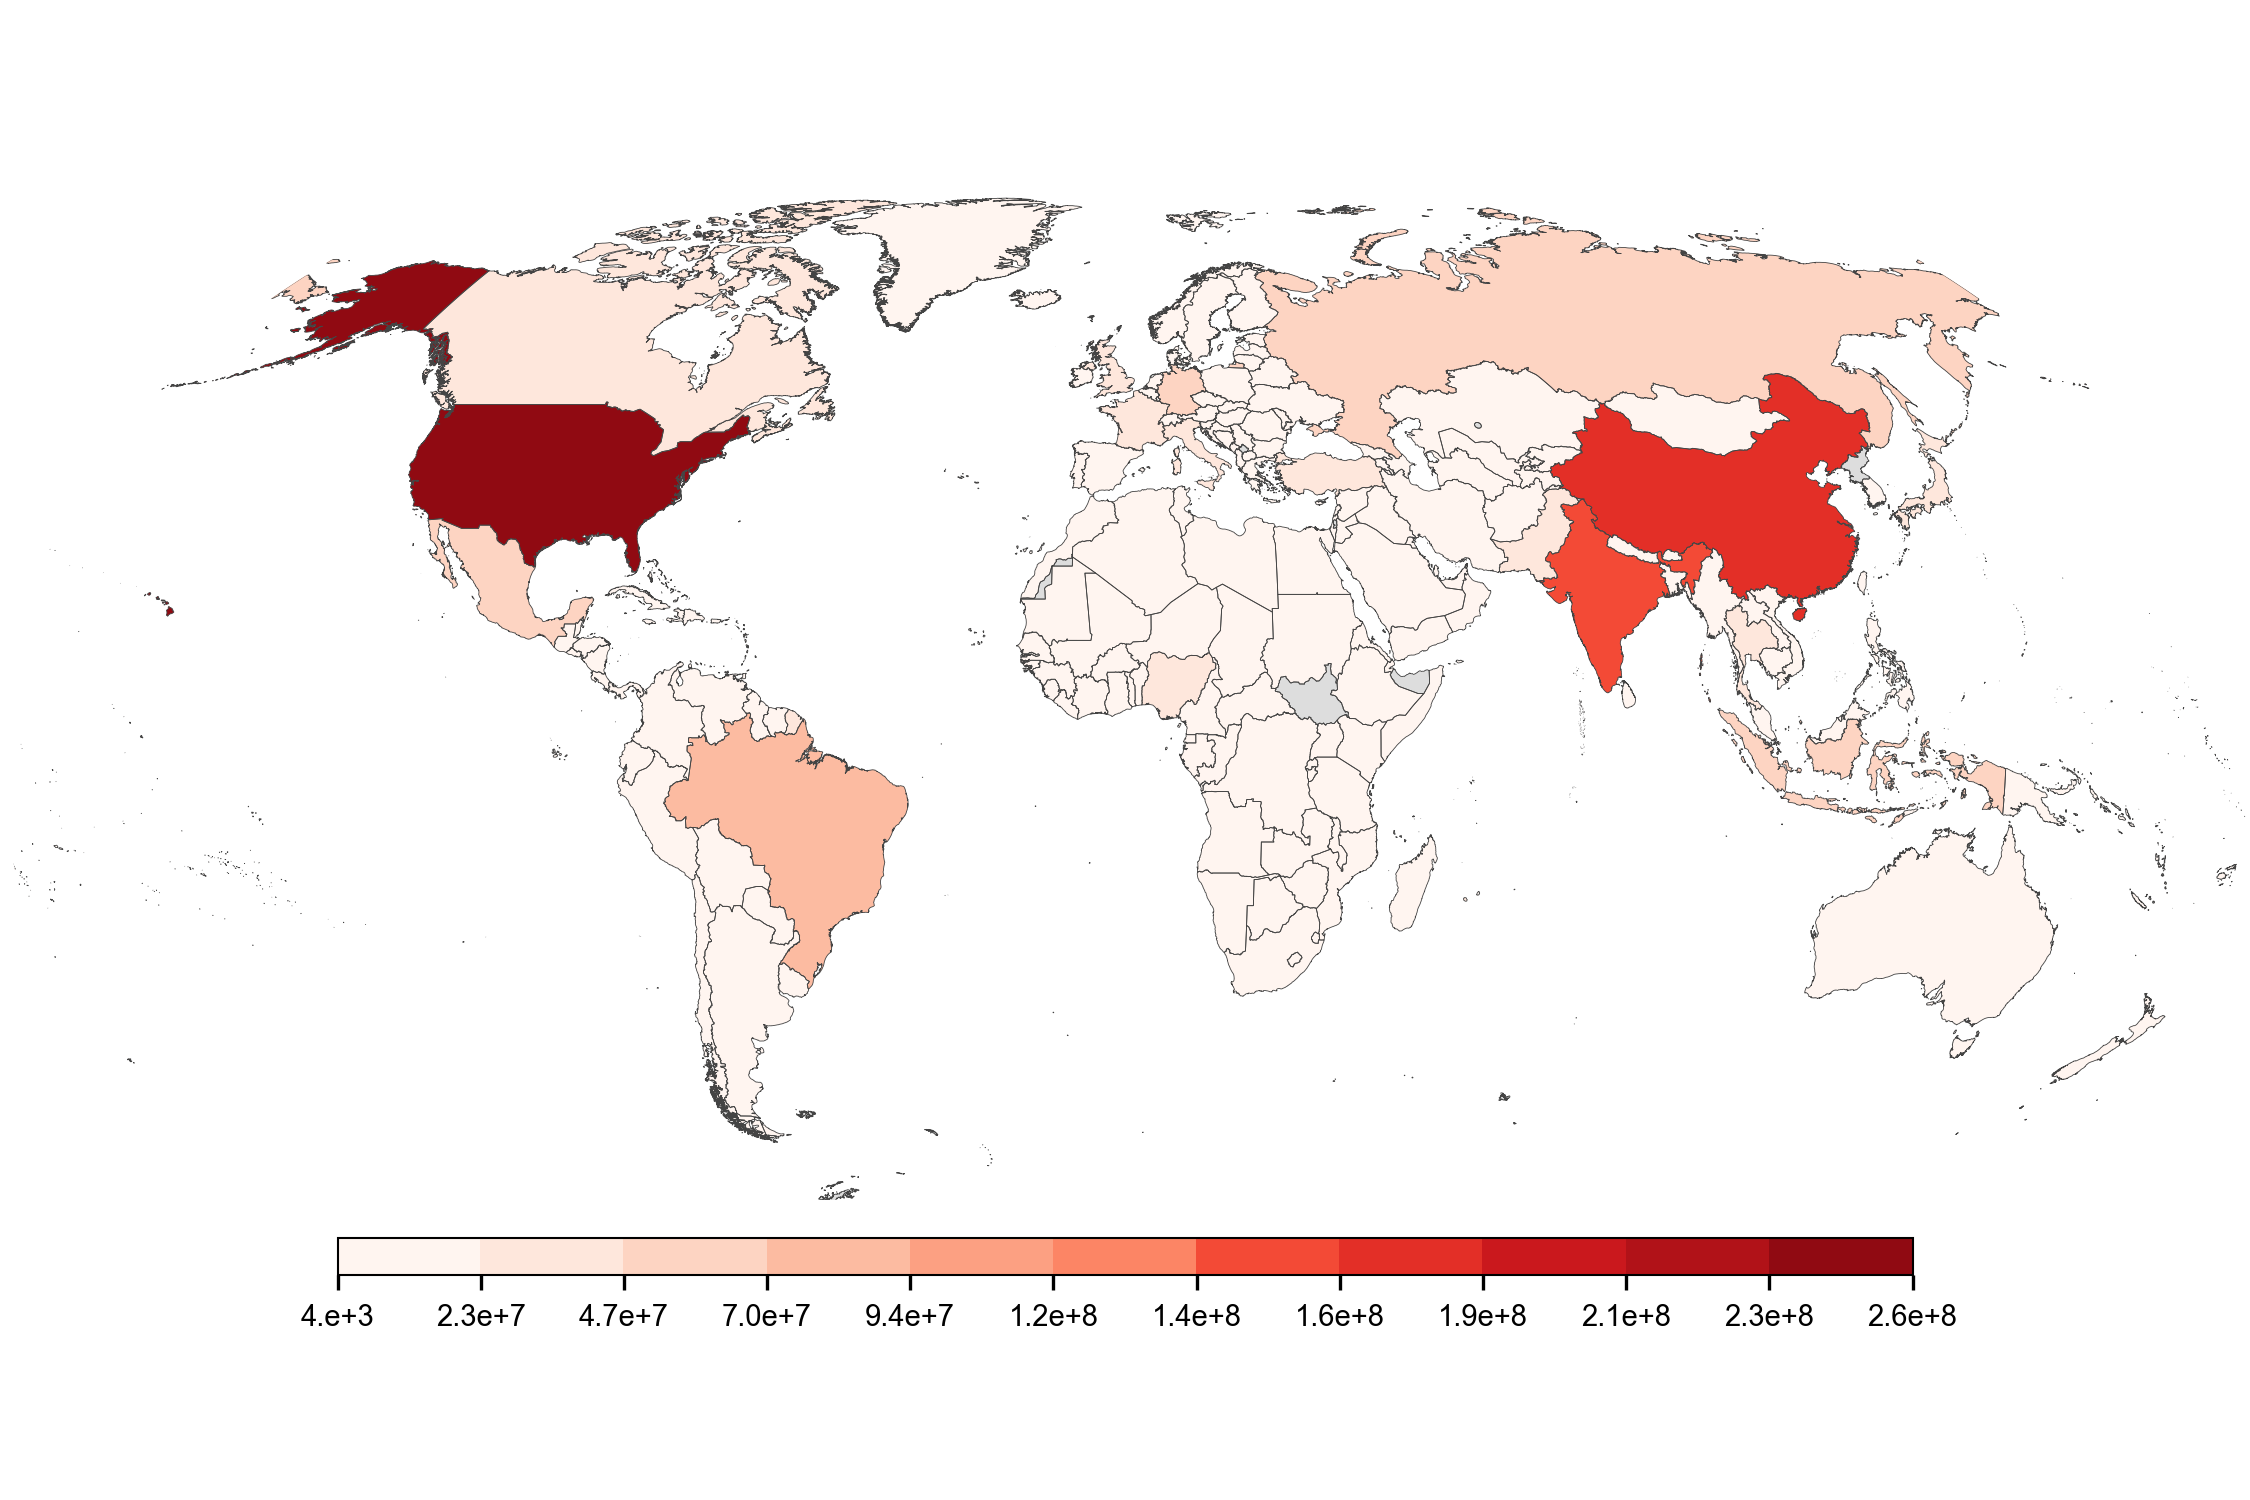
\includegraphics[width=\linewidth]{global-waste-map.png}
	\caption[Waste generated per country, color-coded by quantity (in billions) as of 2018]
	{
		\textbf{Waste generated per country, color-coded by quantity (in billions) as of 2018}\protect\footnotemark.
  }
	\label{figure:preface:global-waste-map}
\end{figure}
\footnotetext{
  data on waste production per country: \url{https://datacatalog.worldbank.org/dataset/what-waste-global-database}
}

The United States, China, and India produced over 600 million tons of waste in 2019~\cite{theworldbank2018}, exceeding the production of the next 20 countries combined. This trend will continue to rise as the world population is expected to grow another 40\%, totaling 9.8 billion by 2050~\cite{unitednations2017}. Fortunately (or unfortunately) the ability to sustain this growing population will be matched by access to the earth's available raw resources. In terms of energy, the earth is projected to have 155 years of processible coal, 51 years for oil, and 65 years for gas given current population and consumption trajectories~\cite{shafiee2008,worldcoalassociation2015}.
Peak production of oil is expected to begin in 2023, and peak production for natural gas, coal, and uranium will occur by 2050~\cite{mason2007}. And despite slowing of Moore's law, the market for electronic goods will continue to rise by 6\% per year until 2024~\cite{robinson2009,hong2015,zionmarket2018}. The world's population and economy is not limited by natural resources or energy requirements. Instead, what may prevent sustainable population and economic growth is the waste produced from all of these processes. Therefore, for sustained growth waste must be managed and mitigated. Unfortunately, policies enacted by individual countries have been ineffective, ultimately transferring responsibilities to NGOs such as the United Nations or the World Health Organization~\cite{elliott2013}. To tackle the continuing buildup of waste there must be an equivalent advancement and scaling of technologies to counteract its global buildup.

%-----------------------------------------------------------------%
% SUBSECTION
%-----------------------------------------------------------------%
\section{Rise of heavy metal waste}
\label{preface:rise-of-heavy-metal-waste}
One of the greatest environmental concerns is the rise and pervasiveness of heavy metal waste. Growing populations and an increase in technological demand have driven the activity of mining and manufacturing of raw materials and electronic goods to unprecedented levels. The result is a surge in environmental heavy metal contaminants such as chromium (\ce{Cr}), copper (\ce{Cu}), arsenic (\ce{As}), cadmium (\ce{Cd}), mercury (\ce{Hg}), and lead (\ce{Pb}), to name a few. For example, Mining of fossil fuels have pulled metals from the Earth's crust to the surface creating tailings that flow into nearby streams and water beds. Similarly, effluent from manufacturing sites are often dumped or left to flow into adjacent soils which contaminate water and agricultural sources~\cite{rattan2005}.
Without any protective barriers, heavy metals eventually return to the public via contaminated water and food. The toxic effects of heavy metals are broad, ranging from gastrointenstinal, epidermal, neurological diseases, cancer, and in acute dosages death (\TABLE~\ref{table:preface:metal-health-stats})~\cite{singh2011}.

Heavy metal waste is becoming more of a concern given the exponential rise in electronic waste (e-waste). Production of e-waste is led by the United States, Europe, and China, generating almost 50 million tons in 2016~\cite{robinson2009,unitednationsuniversity2017}.

%~~~~~~~~~~~~~~~~~~~~~~~~~~~~~~~~~%
% stats on metal hazard
%~~~~~~~~~~~~~~~~~~~~~~~~~~~~~~~~~%
\begin{table}[H]
	\small
	\centering
	\singlespacing
	\def\arraystretch{1.33} % temporary row padding
	\begin{tabular}{l p{4.6cm} p{4.6cm} l}
  \toprule
  \makecell{Metal} & \makecell{Source} & \makecell{Effect} & \makecell{toxic\\level(ppm)}  \\
  \midrule
  Chromium (Cr)
    & mines, chemical industry, metallurgy, dyes and pigments
    & nervous system damage
    & 0.1                              \\
  Manganese (Mn)
    & welding, fuel addition, ferromanganese production
    & damage to central nervous systems
    & 0.05                              \\
  Iron (Fe)
    & naturally occuring in soils, minerals, and the earth's crust. 2nd most abundant metal on the earth's crust
    & plant growth inhibition, corrosion of the gastrointestinal tract, metabolic interference, accumulation in organs
    & 0.3                              \\
  Cobalt (Co)
    & mining, electronic and battery production
    & inhibits DNA repair, genotoxic, dermatitis
    & n/a                              \\
  Nickel (Ni)
    & metal refineries, coins, electronics, battery, and magnet production
    & creates free radicals, haematoxic, neuro and genotoxic
    & 0.1                              \\
  Copper (Cu)
    & mining, pesticides, chemical industry, metal piping
    & anemia, liver, kidney, stomach and intestinal damage
    & 1.3                              \\
  Zinc (Zn)
    & refineries, brass manufacture, metal plating, plumbing
    & skin damage, nervous system
    & 5                                \\
  Arsenic (As)
    & pesticides, fungicides, mteal smelters
    & bronchitis, acute poisoning
    & 0.01                             \\
  Cadmium (Cd)
    & electronics, batteries, nuclear power plants, fertilizers, pesticides
    & Renal damange, lung disease/cancer, bone defects, respiratory damage/cancer, blood, gastrointestinal
    & 0.005                            \\
  Mercury (Hg)
    & pesticides, batteries, lighting, (old) electronics, paper industry
    & tremors, damange to nervous systems, poisoning
    & 0.002                            \\
  Lead (Pb)
    & paint, pesticides, smoking, automobiles, mining, burning fossil fuels
    & mental retardation, development delay, neural diseases, chronic damage to neural, gastro, liver, and kidney
    & 0.015 \\
  \bottomrule
\end{tabular}

	\caption[Sources of heavy metals and their effect on human health]
	{
		\textbf{Sources of heavy metals and their effect on human health}\protect\footnotemark.
	}
	\label{table:preface:metal-health-stats}
\end{table}
\footnotetext{
	table modified from Singh et al., and Jaishankar et al.
	metal permissible as by the EPA: \url{https://www.epa.gov/dwstandardsregulations}
}

\noindent Globally, this is equivalent to 6.5 kilograms (14 pounds) of generated e-waste per person on average; however some countries such as Austrialia have higher generation of e-waste per-capita at 17.3 kg (38 pounds) per person. E-waste is expected to grow another 17\% by 2021, and will lead as the world's fasting growing waste stream~\cite{unitednationsuniversity2017}. Unfortunately, only 20\% is collected or recycled, the remaining 80\% is landfilled or exported to other countries~\cite{schmidt2006,unitednationsuniversity2017}. What this means is that beyond trying to manage already harmful practices such as mining and manufacturing, the advent of electronic waste will only exacerbate the heavy metal waste scenario.

The repurcussions of the rise in heavy metal waste is the toxification of both urban and environmental settings. Heavy metal contamination has disproportionally affected developing countries, especially those in Africa, South America, and the Middle East. Access to unsafe and poorly sanitized living areas have contributed to poisoning and death (\FIGURE~\ref{figure:preface:WHO-death-stats}).
Deaths rates are more concentrated in LICs such as Niger and Chad, whereas the likelihood of deaths related to heavy metal poisoning are less frequent in higher income countries~(\FIGURE~\ref{figure:preface:WHO-death-stats}a).
LMCs and LICs are 10--50\% more likely of heavy metal related death, and since the 2000s the rate of death has either remained constant or increased (\FIGURE~\ref{figure:preface:WHO-death-stats}b).

%=======================================%
% Deaths caused by poor water management
%=======================================%
\begin{figure}[H]
	\centering
	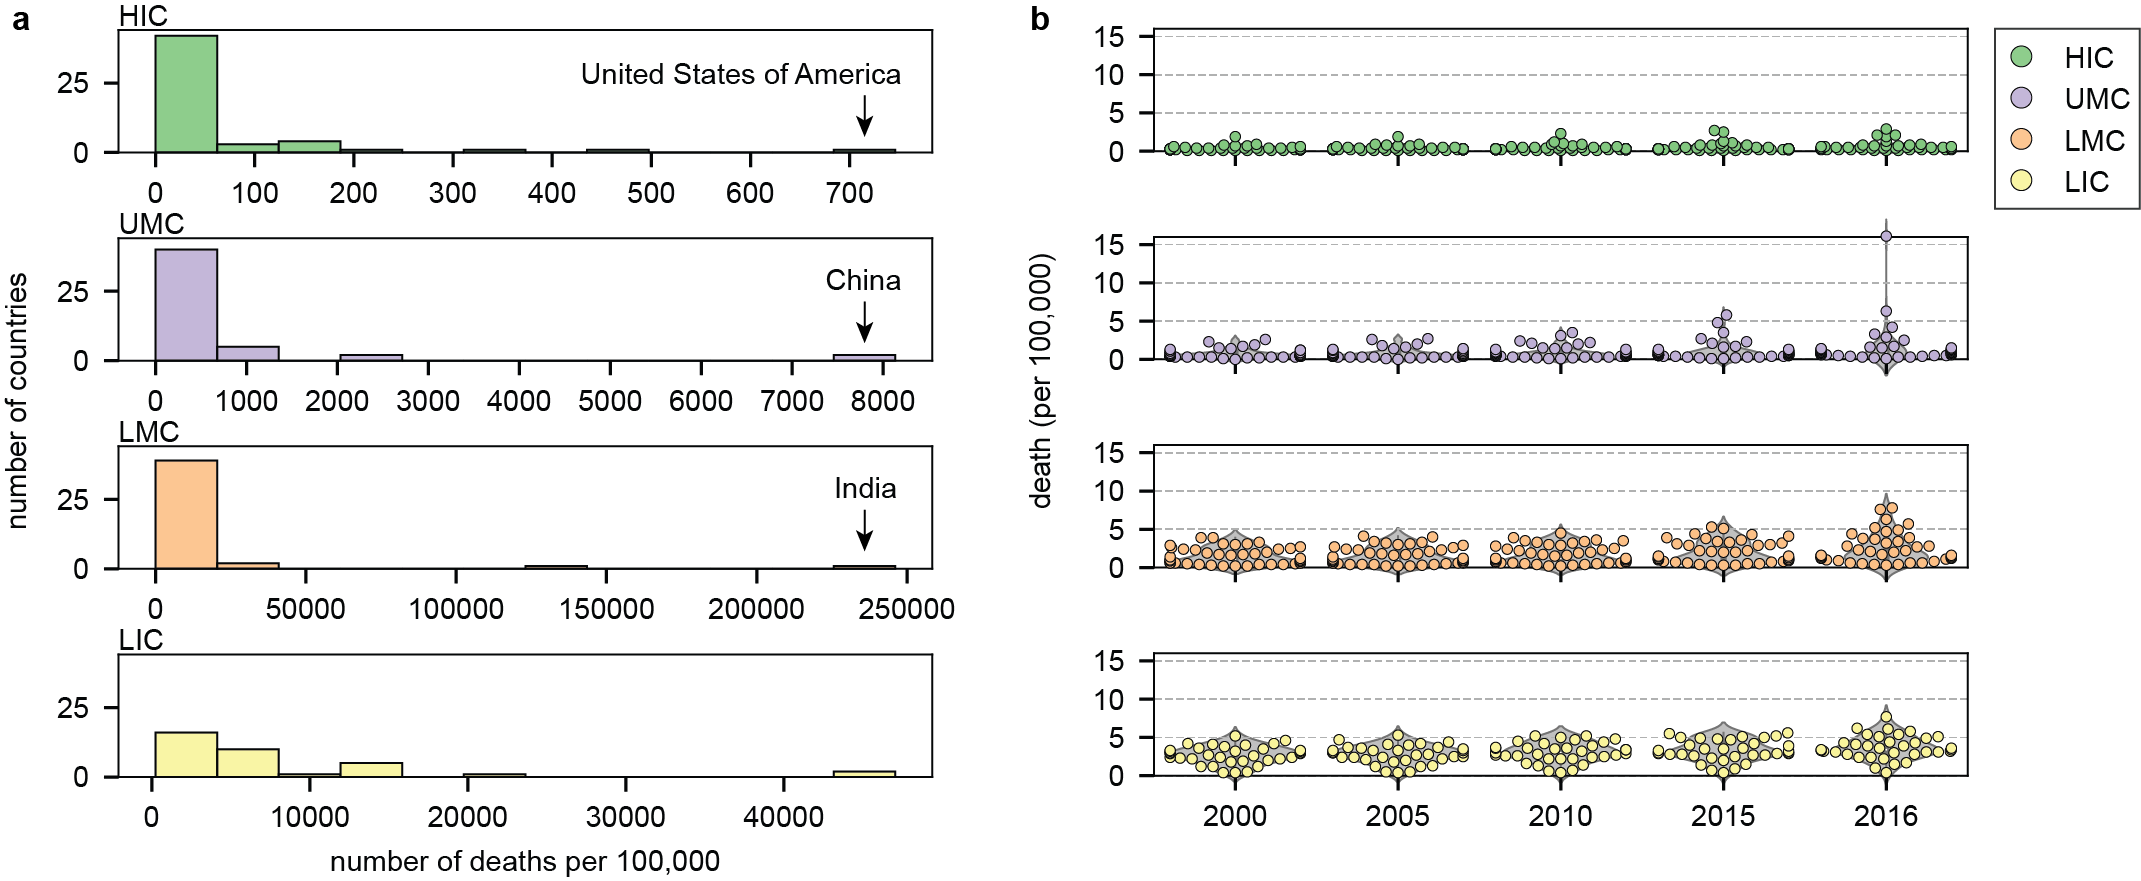
\includegraphics[width=\linewidth]{WHO-death-stats-cropped.png}
	\caption[Deaths related to poor water access linked to heavy metal contamination]
	{
    \textbf{Deaths related to poor water access linked to heavy metal contamination}\protect\footnotemark.
		Death rates per country broken down by economic status (HIC, LIC, LMC, UMC)
    (\textbf{a}) Number of deaths attributed to poor water sanitation.
    (\textbf{b}) Time serie scatter plots of number of deaths since 2000 attributed to poor water sanitation.
  }
  \label{figure:preface:WHO-death-stats}
\end{figure}
\footnotetext{
  data on mortality rate attributed to unsafe waters available at: \url{http://apps.who.int/gho/data/node.main.INADEQUATEWSH?lang=en}\\
  data on global causes of death available at: \url{https://ourworldindata.org/causes-of-death}
}

The rise in heavy metal waste has dramatically impacted the quality and safety of drinking waters. Polluted waters due to heavy metal leaching have starkly increased the number of deaths in the African and South American countries~(\FIGURE~\ref{figure:preface:global-water-sanitation}). About 2.1 billion people lack access to safe drinking waters and more than 4.5 billion, more than half of the world's population, lack managed sanitation services from their community or government~\cite{unitednations2015,unu-inweh2017}.
Again, countries such as the United States and European countries face little sanitation or water accessibility challenges, while the burden is disporportional higher in LMC and LICs~(\FIGURE~\ref{figure:preface:global-water-access}).

%===============================%
% global map of water sanitation
%===============================%
\begin{figure}[H]
	\centering
	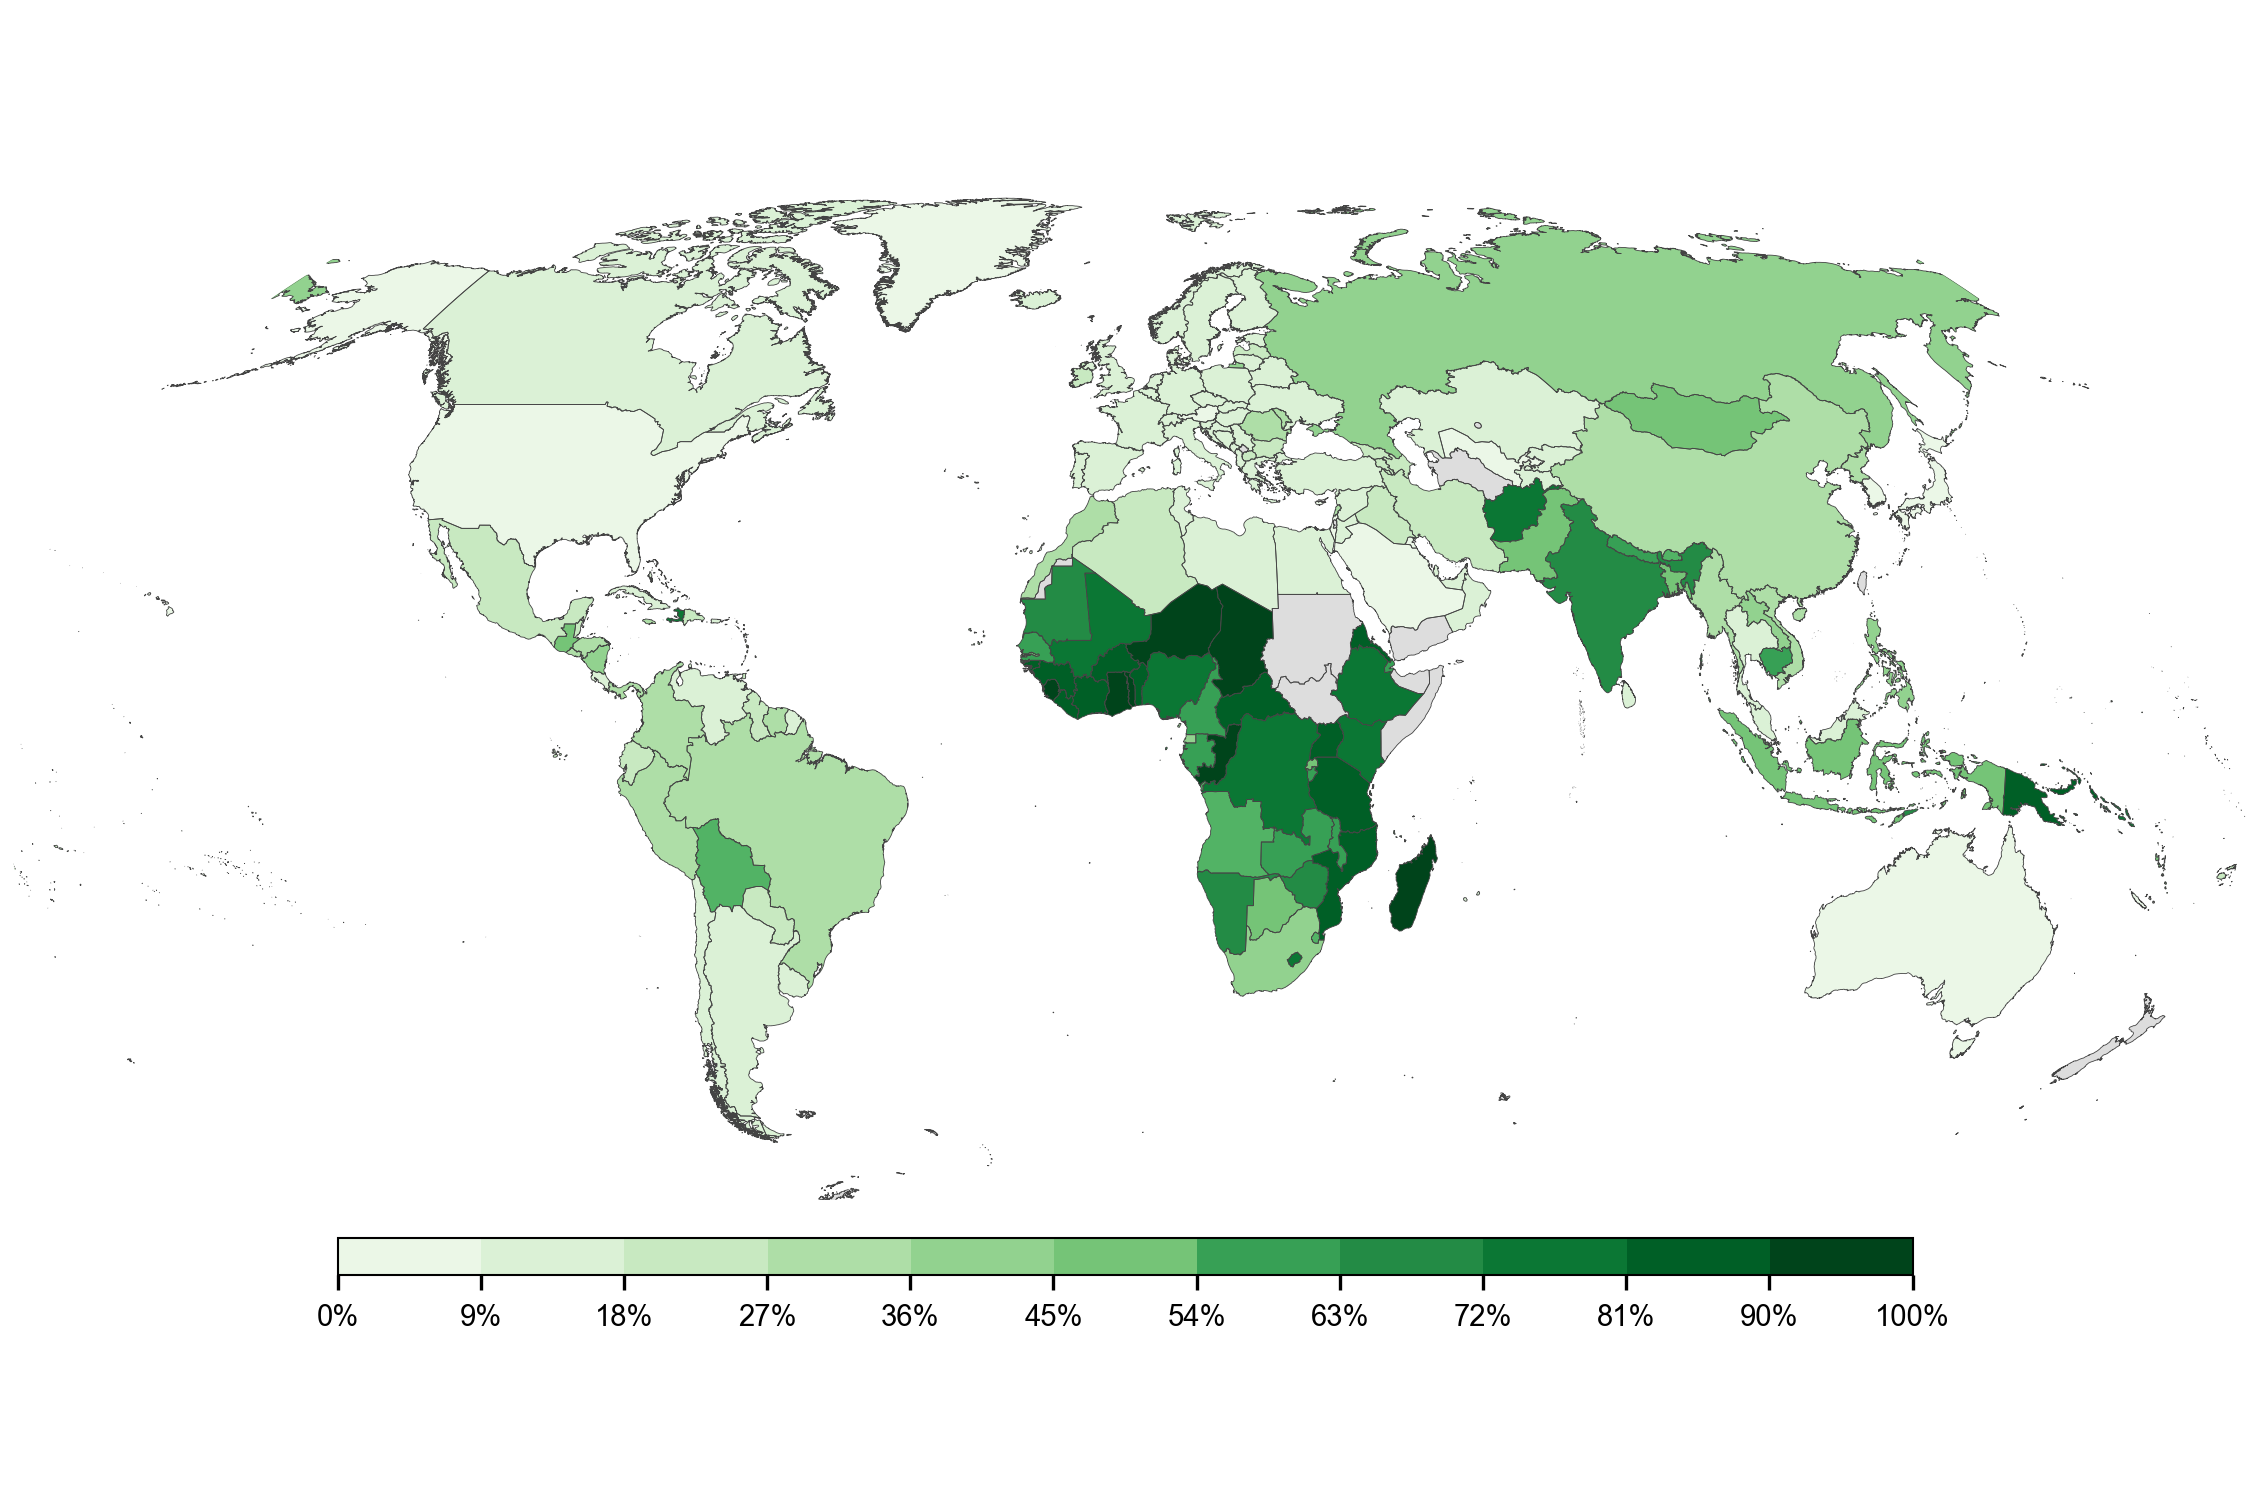
\includegraphics[width=\linewidth]{global-map-sanitation.png}
	\caption[Mortality rate per country due to unsafe water, sanitation, and hygiene services]
	{
		\textbf{Mortality rate per country due to unsafe water, sanitation, and hygiene services}\protect\footnotemark.
		Data from 2016 collected from the World Health Organization. Color map of light-to-dark indicate the rate of death due to exposure or use of unsafe water related sanitation services.
	}
	\label{figure:preface:global-water-sanitation}
\end{figure}
\footnotetext{
  global water sanitation and mortality rate data available at: \url{https://www.who.int/gho/phe/water_sanitation/burden/en/index3.html}
}

%============================%
% global map of water access
%============================%
\begin{figure}[H]
	\centering
	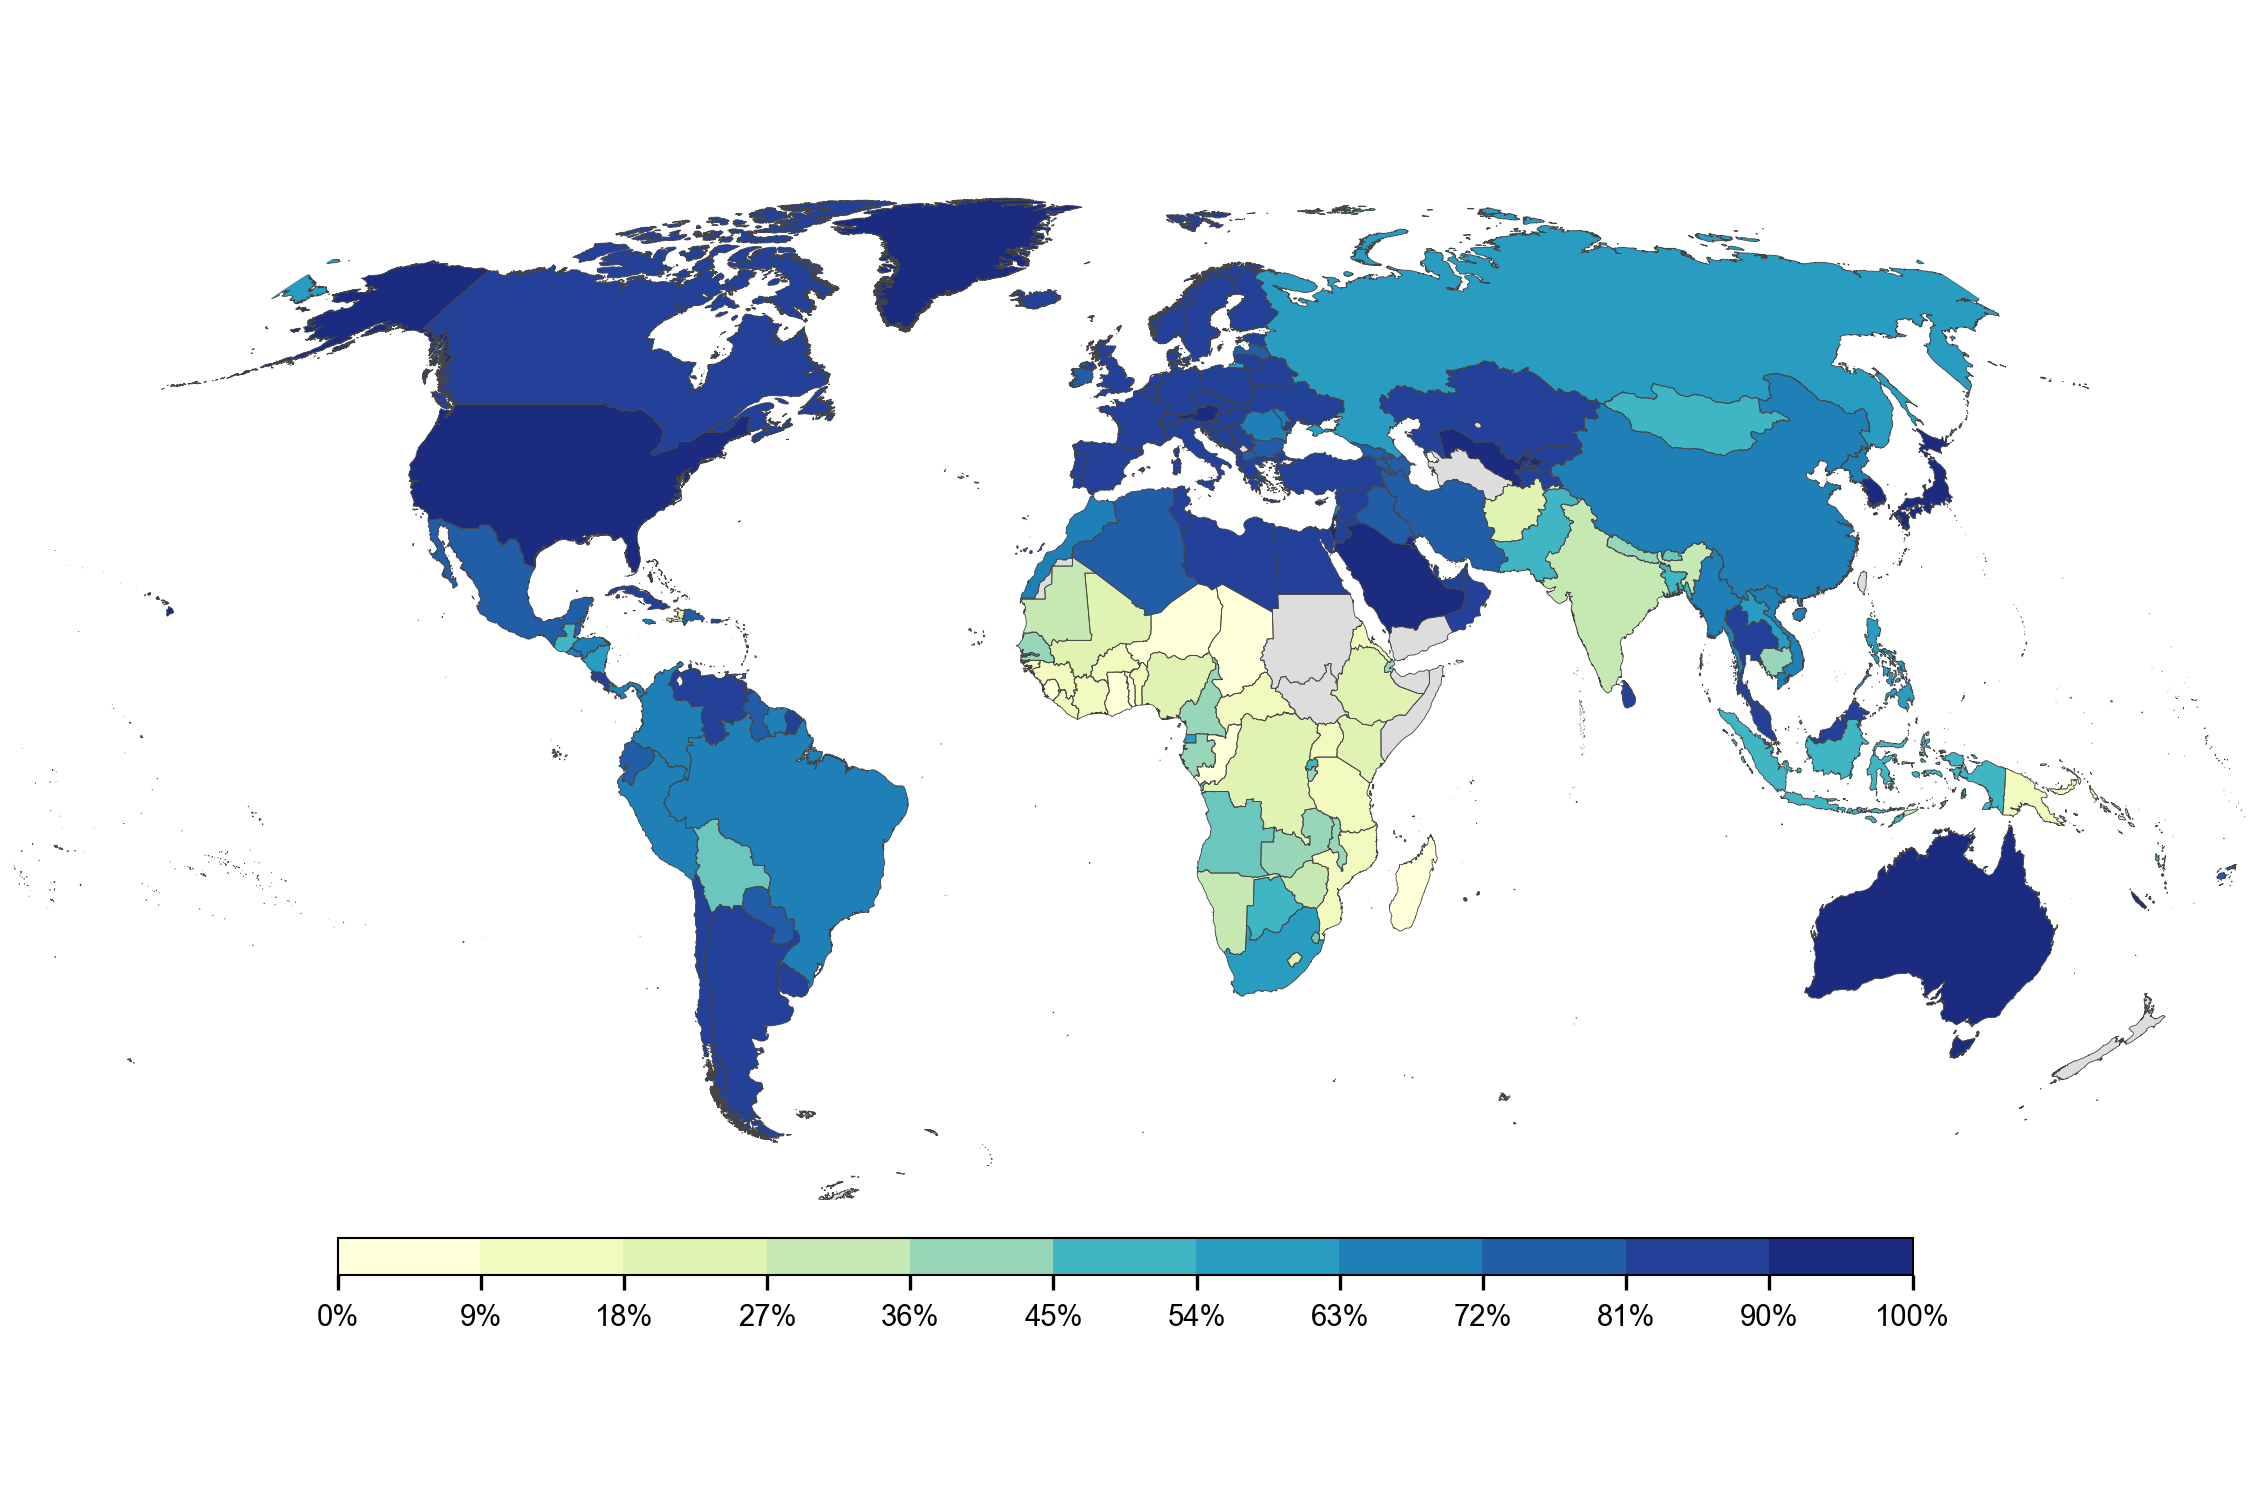
\includegraphics[width=\linewidth]{global-map-access.png}
	\caption[Access to clean water per country]
	{
		\textbf{Access to clean water per country}\protect\footnotemark.
		Almost 850 million people lack access to clean water, many residing in LICs and LMCs.
	}
	\label{figure:preface:global-water-access}
\end{figure}
\footnotetext{
  global water accessibility data available at: \url{https://ourworldindata.org/water-use-sanitation}
}

The abundance of raw materials and energy sources will continue to be available on Earth for the next several decades (\SECTION~\ref{section:preface:current-and-future-trends}). However, water will become increasingly scarce as the remaining drinkable reservoirs are depleted or actively polluted over these next decades. The water burden, calculated by water usage with respect to the available water per country, show that HICs and UMCs are actively draining their water resources faster than any other countries  (\FIGURE~\ref{figure:preface:global-water-burden}).
If this continues, by 2035 more than 40\% of the world will live in seriously water-stressed areas. What makes this situation worse is due to growing population levels and agricultural demand the global need for water will increase by 50\% during this time~\cite{unu-inweh2017}. So not only are countries with low economic power facing extreme water safety challenges, countries with higher economic power are draining the remaining accessible waters at a disproportional rate.

%===========================%
% global map of water burden
%===========================%
\begin{figure}[H]
	\centering
	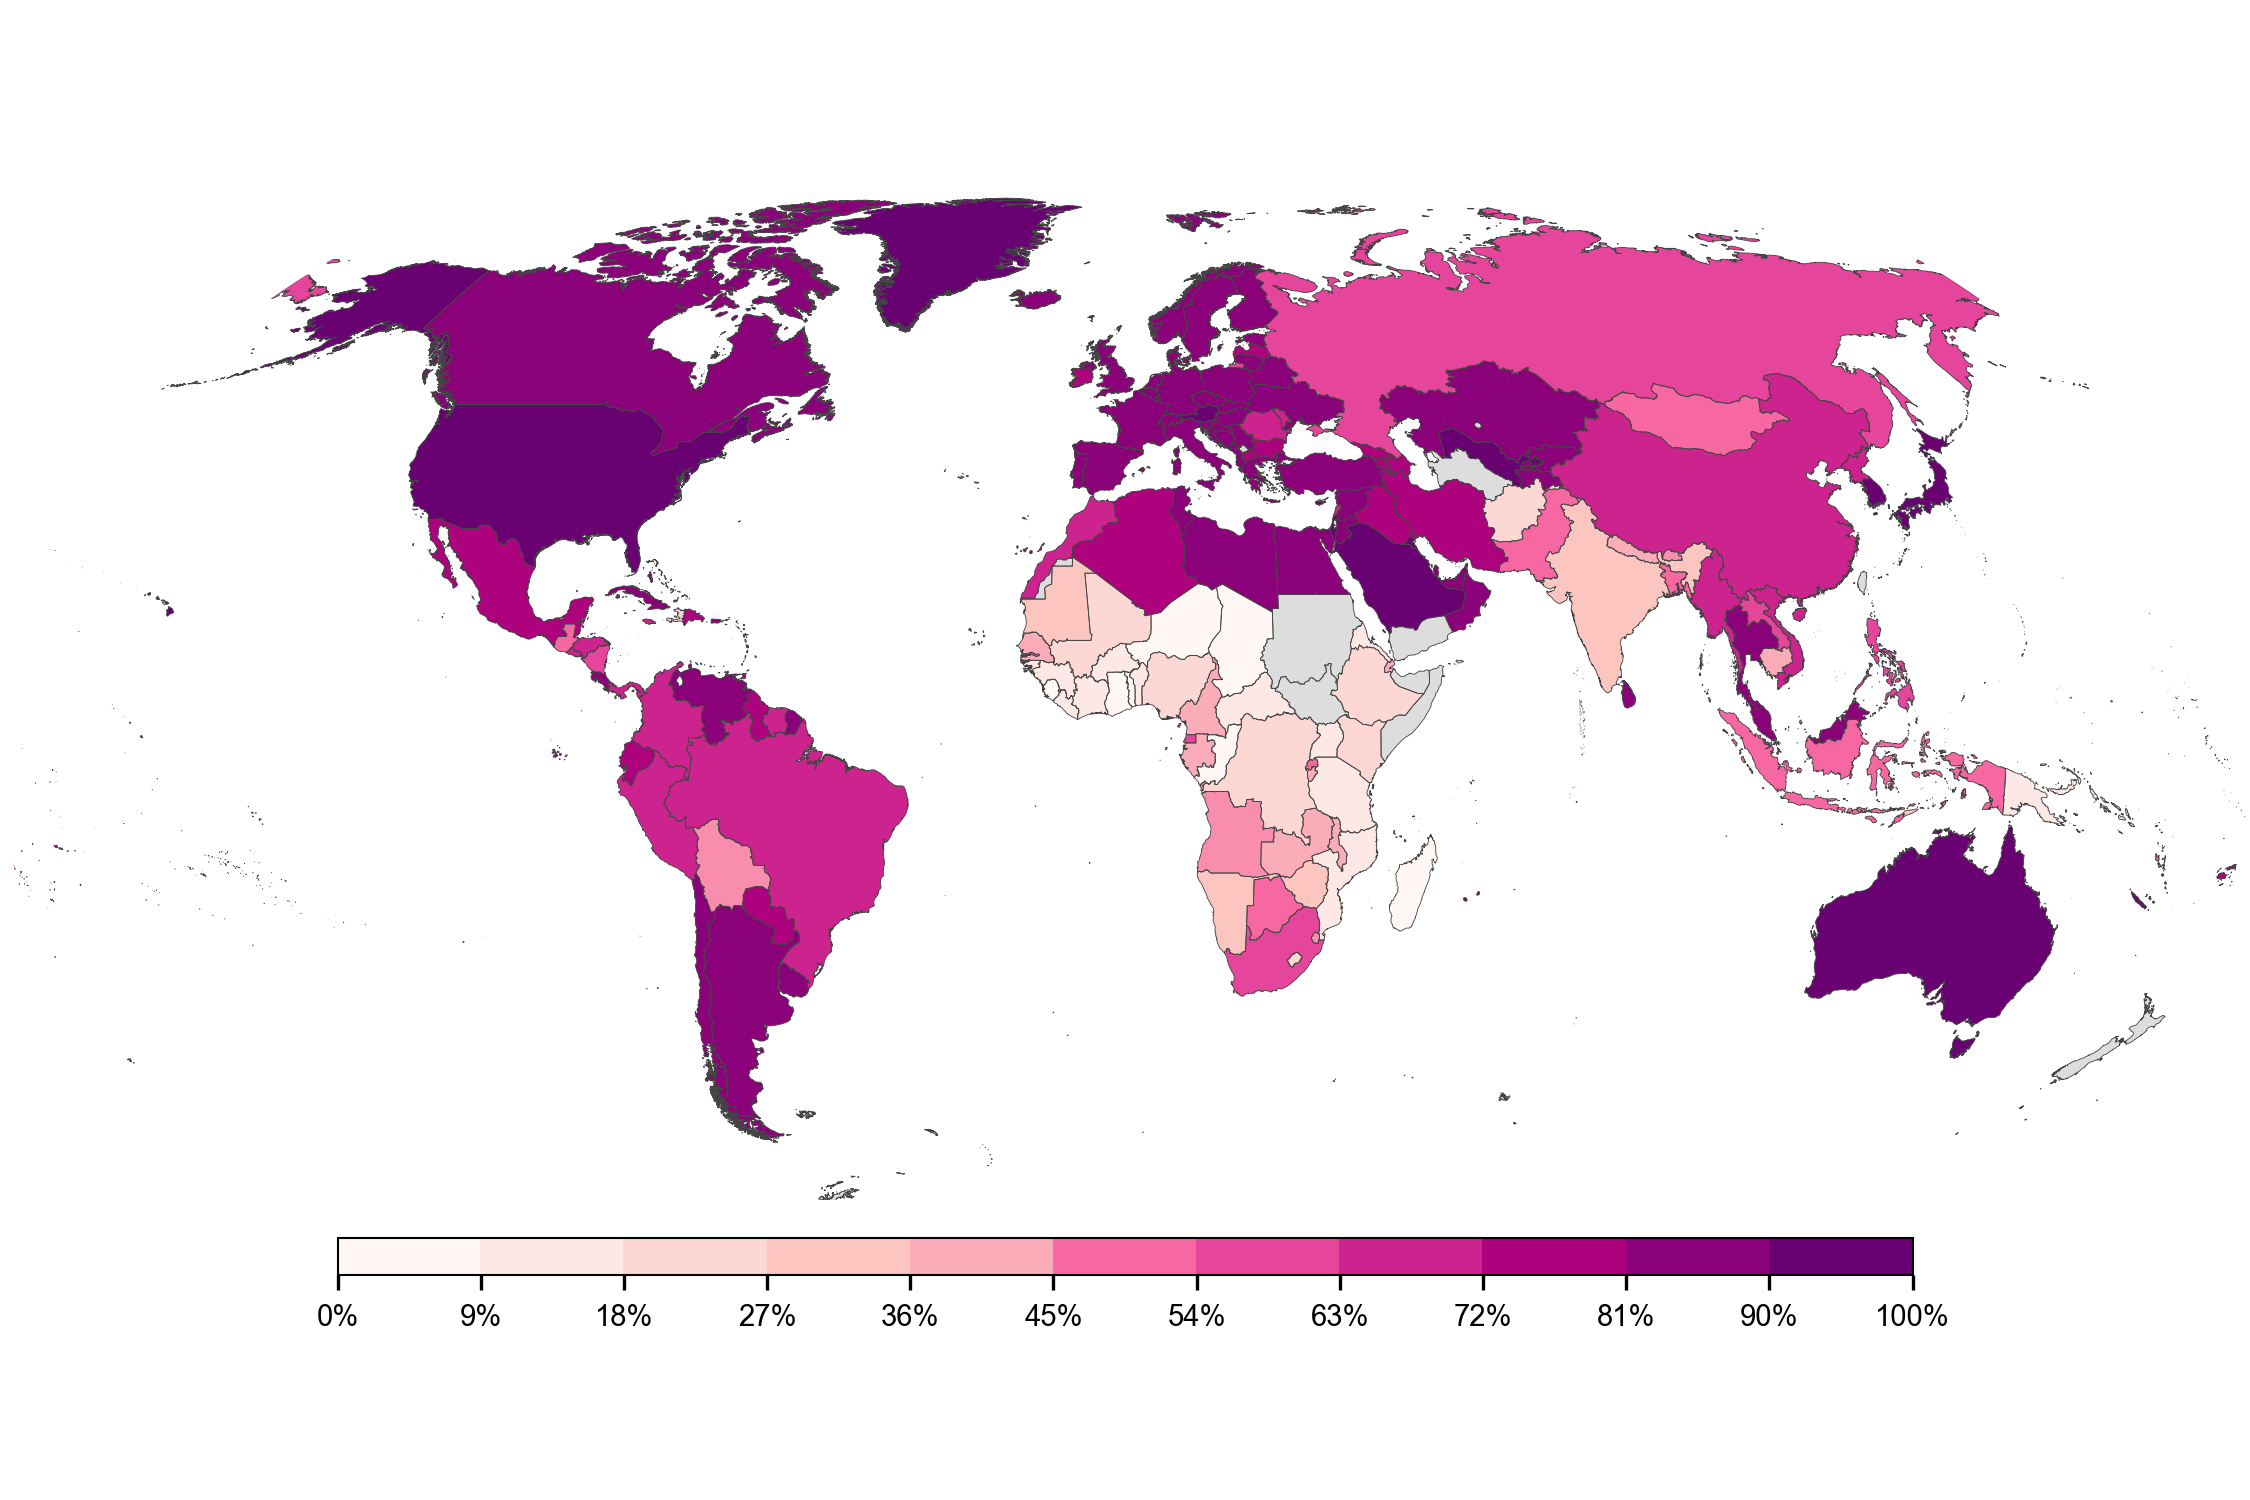
\includegraphics[width=\linewidth]{global-map-burden.png}
	\caption[Percent water usage (i.e. water burden) with respects to the total amount of available water per country]
	{
		\textbf{Percent water usage (i.e. water burden) with respects to the total amount of available water per country}\protect\footnotemark.
	}
	\label{figure:preface:global-water-burden}
\end{figure}
\footnotetext{
  global water usage data available at: \url{https://ourworldindata.org/water-use-sanitation}
}

%===========================================================================%
% SECTION
%===========================================================================%
\section{Concluding remarks}
The rise in waste has resulted in a variety of maladies, from contamination of food and water, health concerns, and ecological damage. However, the negative association surrounding waste is anthropogenically rooted and can be traced back to poor decisions made at the national, government, and public level. However, to blame the public or the government for the current waste scenario is not appropriate or even correct. The purpose of the models and trends described in this work was intended to convey that waste is an inevitable---and arguably a natural---by-product rather than an abhorrent phenomenon. No matter how much pressure is made on the national and international level, humans will continue to make waste. It is inevitable. Instead, if a group or entity should be blamed it should be on the scientific and engineering community. We are responsible for providing our communities with technological answers to difficult questions, and right now that is waste. So far we have performed well in bringing about the Industrial Revolution and now the Silicon and Telecommunication Revolution, but there has only been a murmur in the waste management field. The work herein attempts to motivate a new technological focus on waste remediation and environmental technology. The same manufacturing and technological revolution that has helped push the world into today's new scientific era deserves a complimentary technology to remove, remediate, and recycle the dangerous by-products that come from it.

%===============================BIBLIOGRAPHY================================%
\printbibliography[title=References]

%===================================RESET===================================%
% reset chapters back to 1 for subsequent labelled chapters
\setcounter{chapter}{0}

% change prefix figure numbering/lettering back to arabic
\renewcommand{\thetable}{\arabic{table}}
\renewcommand{\thefigure}{\arabic{figure}}

% prefix section heading
\renewcommand{\thechapter}{\arabic{chapter}}
\renewcommand{\thesection}{\arabic{section}}
\renewcommand{\thesubsection}{\arabic{section}.\arabic{subsection}}

\end{document}
